\documentclass[12pt]{ociamthesis}  % default square logo 
%\documentclass[12pt,beltcrest]{ociamthesis} % use old belt crest logo
%\documentclass[12pt,shieldcrest]{ociamthesis} % use older shield crest logo

%load any additional packages
\usepackage{color}
\usepackage[usenames]{xcolor} 
\usepackage{amssymb,mathrsfs,amsthm,amsmath,lpic,cite,natbib,subfigure,setspace}

\usepackage{tikz}
\usetikzlibrary{arrows,positioning,patterns,decorations.pathreplacing}

\tikzset{
    at xy split/.style 2 args={
        at={(#1,#2)}
    },
    a/.style={circle, draw=red},`'
    b/.style={rectangle, draw=blue}
}

% \includeonly{chapter.State.dependent.disturbance}

%input macros (i.e. write your own macros file called mymacros.tex 
%and uncomment the next line)
%\include{mymacros}


% \includeonly{app.PDE}


\title{Robust Model Predictive Control}   %note \\[1ex] is a line break in the title

\author{Rainer Manuel Schaich}             %your name
\college{Worcester College}  %your college

%\renewcommand{\submittedtext}{change the default text here if needed}
\degree{Doctor of Philosophy}     %the degree
\degreedate{Hilary 2017}         %the degree date

%end the preamble and start the document
% \usepackage{showkeys}

\colorlet{lcolor}{blue!40!black}
\colorlet{ucolor}{magenta!40!black}
\colorlet{ccolor}{green!40!black}

\usepackage[colorlinks=true,%
            linkcolor=lcolor,%
            urlcolor=ucolor,%
            citecolor=ccolor]{hyperref}
\hypersetup{pdfauthor={Manuel Schaich},hidelinks=true}

\graphicspath{{./Pix/}}

\providecommand{\norm}[1]{\left\|#1\right\|}
\providecommand{\abs}[1]{\left|#1\right|}
\providecommand{\span}{\text{span}}
\providecommand{\conv}{\text{conv}}
\providecommand{\rk}[1]{\text{rank}\left(#1\right)}

\newcommand*{\Resize}[1]{\resizebox{\columnwidth}{!}{$#1$}}

\newcounter{thmcount}[chapter]
\renewcommand{\thethmcount}{\thechapter.\arabic{thmcount}}
\renewcommand{\theequation}{\thechapter.\arabic{equation}}
\renewcommand{\thefigure}{\thechapter.\Roman{figure}}


% \newcounter{subeq}[equation]
% \renewcommand{\thesubeq}{\theequation.\roman{subeq}}
% \newcommand{\subeqcount}[1]{\refstepcounter{subeq}\thesubeq\label{#1}}

\makeatletter 
\def\mynobreakpar{\par\nobreak\@afterheading} 
\def\mynobreakline{\par\nobreak\vspace{-\parskip}\@afterheading\noindent} 
\makeatother

\newenvironment{thm}[1][]%
{\refstepcounter{thmcount}\par\noindent\textbf{Lemma \thethmcount} \textsc{#1}\mynobreakpar%
\begin{tabular}{|p{0.98\textwidth}} \it}%
{\end{tabular}\par\noindent}

\newenvironment{korr}%
{\refstepcounter{thmcount}\par\noindent\textbf{Corollary \thethmcount}\mynobreakpar%
\begin{tabular}{|p{0.98\textwidth}} \it}%
{\end{tabular}\par\noindent}

\theoremstyle{remark}
\newtheorem{rem}[thmcount]{Remark}

\newenvironment{ass}%
{\refstepcounter{thmcount}\par\noindent\textbf{Assumption \thethmcount\;}%
\newline}%
{\par\noindent}

\newenvironment{blanko}[1][]%
{\refstepcounter{thmcount}\vspace{1em}\noindent\textbf{#1 \thethmcount\;}\textsc{#1}\mynobreakpar}%
{\par\noindent}


\newenvironment{defn}[1][]%
{\refstepcounter{thmcount}\par\noindent\textbf{Definition \thethmcount} \textsc{#1}%
\mynobreakpar%
\begin{tabular}{|p{0.98\textwidth}} \it}%
{\end{tabular}\vspace{1em}\noindent}


\DeclareFontFamily{U}{mathx}{\hyphenchar\font45}
\DeclareFontShape{U}{mathx}{m}{n}{
      <5> <6> <7> <8> <9> <10> gen * mathx
      <10.95> mathx10 <12> <14.4> <17.28> <20.74> <24.88> mathx12
      }{}
\DeclareSymbolFont{mathx}{U}{mathx}{m}{n}
\DeclareFontSubstitution{U}{mathx}{m}{n}
\DeclareMathSymbol{\temp}{\mathbin}{mathx}{'341}
\newcommand{\bigominus}{\raisebox{10pt}{$\temp$}}


\begin{document}
%this baselineskip gives sufficient line spacing for an examiner to easily
%markup the thesis with comments
\baselineskip=18pt plus1pt

%set the number of sectioning levels that get number and appear in the contents
\setcounter{secnumdepth}{3}
\setcounter{tocdepth}{3}

\maketitle    

\begin{romanpages}          % start roman page numbering
\tableofcontents            % generate and include a table of contents
\listoffigures              % generate and include a list of figures
\end{romanpages}            % end roman page numbering

% \doublespace
%!TEX root = main.tex

\chapter{Introduction}

\section{Notation}
%
By $A\vert_B$ we denote $A$ evaluated on $B$.
%!TEX root = main.tex

% %
% We denote trajectories of the disturbance and input by~${\bf{w}}=(w_0,\dots,w_{N-1})\in\mathcal W^N$ and 
% ${\bf{u}} = (u_0,\dots,u_{N-1})\in\mathcal U^N$ respectively, the resulting state trajectory is then denoted 
% by~${\bf{x}}^{\bf{u},\bf{w}}(x_0) = (x_0,f(x_0,u_0,w_0),\dots)$
% %
% For notational convenience we denote by~$x_i$ the $i$-th state of the optimal state trajectory for
% the performance criterion
% %
% \begin{equation}\label{eq:concepts:general:objective:no:term:cost}
% 	J_m(x_{m}) = \min_{u_{m}\in\mathcal U}\max_{w_{m}\in\mathcal W} l(x_{m},u_{m}) - \gamma(w_{m}) + J_{m-1}(x_{m+1}),
% \end{equation}
% %
% i.e. $x_i$ is the $i$-th column of the optimal state trajectory~${\bf{x}}^{\bf{u}^\ast,\bf{w}^\ast}(x_0)$
% with the optimisers~${\bf{u}}^\ast$ and~${\bf{w}}^\ast$.
% %
% We assume that we have $\mathcal K^\infty$ functions $\alpha_i, i\in\{1,\dots,8\}$ such that
% %
% \begin{subequations}
% \begin{equation}
% 	\alpha_1(\norm{x}) + \alpha_2(\norm{u}) \leq l(x,u) \leq \alpha_3(\norm{x}) + \alpha_4(\norm{u})
% \end{equation}
% and
% \begin{equation}
% 	\alpha_5(\norm{w})\leq\gamma(w)\leq\alpha_6(\norm{w}).
% \end{equation}
% \end{subequations}
% %
% Furthermore we assume that $l(x,u)$ and $\gamma(w)$ are convex in $u\in\mathcal U$ and $w\in\mathcal W$
% respectively.
% %
% To initialise the recursion we use $J_0(x) = V(x)$ as the unconstrained infinite horizon solution
% %
% \begin{equation}
% 	V(x_0) = \lim_{N\rightarrow\infty} \min_{u_0}\max_{w_0}\dots \min_{u_{N}}\max_{w_{N}}\sum_{i=0}^{N}l(x_i,u_i)-\gamma(w_i)
% \end{equation}
% %
% its optimal solution is given by
% %
% \begin{equation}
% 	\bigl(\kappa(x),\nu(x,\kappa(x)\bigr) = \arg\min_{u_0,\dots}\max_{w_0,\dots} \sum_{i=0}^\infty l(x_i,u_i) - \gamma(w_i)
% \end{equation}
% %
% notice that this implies
% \begin{gather}
% 	V(x_0) = \min_{u_0}\max_{w_0} l(x_0,u_0)-\gamma(w_0) + V(f(x_0,u_0,w_0))\geq 
% \end{gather}
% %
% \begin{gather}
% 	\alpha_7(\norm{x}) \leq V(x) \leq \alpha_8(\norm{x}) \nonumber \\
% 	V(f(x,\kappa(x),w))-V(x) \leq -l(x,\kappa(x)) + \gamma(w)\label{eq:concepts:ISS:property:general}
% \end{gather}
% %
% for the unconstrained optimal infinite horizon controller~$u = \kappa(x)$, i.e. $\kappa$ satisfies 
% %
% if it exists.
% %
% Notice that~\eqref{eq:concepts:ISS:property:general} implies that $V(x)$ is an \emph{ISS-Lyapunov function} 
% for $x^+=f(x,\kappa(x),w)$ (see~\cite{Jiang:2001}), since
% %
% \begin{equation}
% 	\eqref{eq:concepts:ISS:property:general}\leq -(\alpha_1(\norm{x})+\alpha_2(\norm{\kappa(x)})) + \alpha_6(\norm{w})
% \end{equation}
% %
% and in particular
% %
% \begin{equation}
% 	V(f(x,\kappa(x),w))-V(x) \leq -\alpha_1(\norm{x}) + \alpha_6(\norm{w}).
% \end{equation}


% Like in nominal MPC algorithms the controller that is applied to the system is given by~$u=u_0^\ast$, so that
% the subsequent problem is then to solve~\eqref{eq:concepts:general:objective:no:term:cost} for the current 
% state~$f(x_0,u_0^\ast,\hat w_0)$ for the actual realisation $\hat w_0\in\mathcal W$.

\chapter{Concepts of Robust Model Predictive Control}\label{chap:concepts}
%
In this chapter we cover the main concepts which make up the foundation of
the robust model predictive control (RMPC) schemes we will discuss later on.
%
We present the concepts as general as possible and will only exploit special 
structures if necessary.
%

%
First we examine the unconstrained infinite horizon problem for a given discrete time system 
%
\begin{equation}\label{eq:concepts:general:system}
 	x_{i+1} = f(x_i,u_i,w_i)
\end{equation} 
%
with the state $x\in\mathbb R^n$, the control input $u\in\mathbb R^{n_u}$ and the disturbance 
input $w\in\mathbb R^{n_w}$ we seek to optimally steer the system state~$x$ from the initial state $x_0$ to the the 
equilibrium $0 = f(0,0,0)$ with respect to the performance criterion
%
\begin{equation}\label{eq:concepts:infinite:horizon:problem}\begin{split}
	V(x) = &\lim_{N\rightarrow\infty} \min_{u_0}\max_{w_0}\dots\min_{u_N}\max_{w_N} \sum_{i=0}^N l(x_i,u_i)-\gamma(w_i)\\
	&\text{s.t.}\quad\begin{array}{rcl}
	x_{i+1} &=& f(x_i,u_i,w_i)\\
	x_0 &=& x.
	\end{array}
\end{split}\end{equation}
%
We assume that the stage-cost terms can be bounded by the $\mathcal K^\infty$ functions $\alpha_i, i\in\{1,\dots,6\}$
%
\begin{subequations}
\begin{equation}
	\alpha_1(\norm{x}) + \alpha_2(\norm{u}) \leq l(x,u) \leq \alpha_3(\norm{x}) + \alpha_4(\norm{u})
\end{equation}
and
\begin{equation}
	\alpha_5(\norm{w})\leq\gamma(w)\leq\alpha_6(\norm{w}).
\end{equation}
\end{subequations}
%
and by~$u^\ast = \kappa(x)$ and $w^\ast = \nu(x,u)$ we denote the optimal solution to the unconstrained problem
%
Notice that we have
%
\begin{equation}\begin{split}
	V(x) &= \lim_{N\rightarrow\infty} \min_{u_0}\max_{w_0}\dots\min_{u_N}\max_{w_N} \sum_{i=0}^N l(x_i,u_i)-\gamma(w_i)\\
	&\geq \min_{u_0} l(x_0,u_0)-\gamma(w_0^\prime) + \lim_{N\rightarrow\infty}\min_{u_1}\dots\max_{w_N}\sum_{i=1}^N l(x_i,u_i)-\gamma(w_i)\\
	&\vdots\\
	&\geq\lim_{N\rightarrow\infty}\min_{u_0,\dots,u_N}\sum_{k=0}^N l(x_k,u_k)-\gamma(w_k^\prime)
\end{split}\end{equation}
%
where the sequence of $\{w_k^\prime\}$ is chosen arbitrarily, notice further that $\gamma(0)=0$ and $0\geq-\sum_{k=0}^N\gamma(w_k)$.
%
Hence, we have
%
\begin{equation}\begin{split}
	V(x)\geq \tilde V(x) &= \lim_{N\rightarrow\infty}\min_{u_0,\dots,u_N}\sum_{k=0}^N l(x_k,u_k)\\
	&\text{s.t.}\quad\begin{array}{rcl}
	x_{k+1} &=& f(x_k,u_k,0)\\
	x_0 &=& x
	\end{array}
\end{split}\end{equation}
%
which corresponds with the nominal unconstrained optimal control problem, for which we know that we have
%
\begin{equation}\label{eq:concepts:lower:bound:on:inf:cost}
	\beta_1(\norm{x})\leq\tilde{V}(x)\leq V(x)
\end{equation}
%
for some~$\beta_1\in\mathcal K^\infty$. 
%
We assume that there exists an upper bound $V(x)\leq\beta_2(\norm{x})$ with $\beta_2\in\mathcal K$.
%
It follows that~$V$ is an ISS-Lyapunov function for $x^+ = f(x,u^\ast,w) =: F(x,w)$ with $w\neq w^\ast$ (see~\cite{Jiang:2001}):
%
\begin{equation}\begin{split}
	V(x) = l(x,u^\ast)-\gamma(w^\ast) + V(f(x,u^\ast,w^\ast)) \overset{w\neq w^\ast}{\geq} 
	l(x,u^\ast)-\gamma(w) + V(f(x,u^\ast,w))
\end{split}\end{equation}
%
or equivalently
%
\begin{equation}\label{eq:concepts:ISS:condition:cost:to:go}
	V(f(x,u^\ast,w)) - V(x) \leq -l(x,u^\ast) + \gamma(w) \leq - \alpha_1(\norm{x}) + \alpha_5(\norm{w}).
\end{equation}
%
It is known that the existence of a ISS Lyapunov function~$V$ implies that the unconstrained controlled 
uncertain system $x^+ = F(x,w)$ is input-to-state stable (see~\cite{Jiang:2001}).

The robust model predictive control problem we intend to solve is a finite horizon, constrained min-max
optimal control problem.
%
We denote the state constraints~$x\in\mathcal X\subseteq\mathbb R^n$, the input constraints~$u\in\mathcal U\subset\mathbb R^{n_u}$
and the disturbance constraints~$w\in\mathcal W\subset\mathbb R^{n_w}$, we assume that all constraint sets~$\mathcal X,
\mathcal U$ and $\mathcal W$ are convex and closed, furthermore we assume that $\mathcal U$ and $\mathcal W$ are bounded and
hence compact.
%
The RMPC problem is then given by the recursive min-max problems
%
\begin{subequations}
\begin{equation}
	J_m(x_{N-m}) = \min_{u_{N-m}\in\mathcal U}\max_{w_{N-m}\in\mathcal W} l(x_{N-m},u_{N-m})-\gamma(w_{N-m}) + J_{m-1}(x_{N-m+1})
\end{equation}
subject to
\begin{equation}
	x_{i+1} = f(x_i,u_i,w_i)
\end{equation}
\begin{equation}
	x_{N-m},x_{N-m+1}\in\mathcal X
\end{equation}
\end{subequations}
%
which is initialised with the unconstrained solution $J_0(x) = V(x)$, and the system state at the $N$-th stage~$x_N=x$.
%
The robust model predictive control input is then given by~$u_N^\ast$, i.e. the optimal control law at the~$N$-th stage, 
so that the successor state is then given by~$x^+ = f(x,u_N^\ast,\tilde w)$ for some realisation $\tilde w\in\mathcal W$.


In order to guarantee the feasibility of the optimisation problem for all possible realisations of the 
uncertainty~$w\in\mathcal W$ we design state constraints for each stage such that the satisfaction 
of state constraints is guaranteed for all realisations of the uncertainty.
%
Similar to nominal MPC we use a terminal set approach, i.e. the terminal state is constrained to a set
in which~$\kappa(x)\in\mathcal U$ is feasible and renders the set invariant, see e.g.~\citet{Mayne:2000}.
%
However, in the robust setup we require the terminal set to be invariant for all possible realisations of the 
uncertainty, i.e. a set which is invariant under all possible realisations of the closed-loop 
system~$f(x,\kappa(x),w), w\in\mathcal W$, these sets are called \emph{robust positive invariant} (RPI) sets.
%
In particular we use the \emph{largest} RPI set, i.e. the RPI set that contains all \emph{smaller} RPI sets, the
so called \emph{maximal robust positive invariant} (MRPI) set, see~\cite{blanchini:2007} for an elaborate discussion.
%
\begin{defn}[Maximal Robust Positive Invariant Set]\label{def:concepts:MRPI:sets:general}
For an uncertain constrained system $x^+ = F(x,w)$ with $x\in\mathscr X$ and $w\in\mathscr W$
the maximal robust positive invariant set~$\mathcal X^\infty$ is defined as the largest set satisfying
%
\begin{equation}
	\mathcal X^\infty = \left\{x\in\mathcal X : F(x,w)\in\mathcal X^\infty\;\forall\;w\in\mathscr W \right\}
\end{equation}
%
\end{defn}
%
In the case of a terminal set for a RMPC problem we would use~$F(x,w) = f(x,\kappa(x),w)$ and 
$\mathscr X = \{x\in\mathcal X:\kappa(x)\in\mathcal U\wedge \nu(x,\kappa(x))\in\mathcal W\}$.
%
However, simply adding the constraint $x_N\in\mathcal X^\infty$ to the min-max 
recursion~\eqref{eq:concepts:general:objective:no:term:cost} is not enough to guarantee the feasibility of 
the problem, since there might be realisations ${\bf{w}}^\prime\neq{\bf{w}}^\ast$ such that the terminal
state~$x^{\bf{u}^\ast,\bf{w}^\prime}_N(x_0)\not\in\mathcal X^\infty$.
%
For this purpose we constrain the state to the $m$-step \emph{robust controllable sets} $x_m\in\mathcal Z_m$ at 
the $m$-th stage, which is a recursively defined sequence of sets leading towards the MRPI set~$\mathcal X^\infty$,
i.e.
%
\begin{subequations}\label{eq:concepts:def:stage:constraints}
\begin{equation}
	\mathcal Z_m = \{(x,u)\in\mathcal X\times\mathcal U: f(x,u,w)\in\mathcal X_{m-1}\forall\,w\in\mathcal W\}
\end{equation}
%
and its projection
%
\begin{equation}
	\mathcal X_m = \{x\in\mathcal X:\exists\;u\in\mathcal U\;(x,u)\in\mathcal Z_m\}
\end{equation}
initialised with the MRPI set $\mathcal X_0=\mathcal X^\infty$.
\end{subequations}
%
So that the state constrained MRPC problem is given by
%
\begin{subequations}\label{seq:concepts:general:RMPC:problem:with:state:constraints}
\begin{equation}
	J_m(x_{m}) = \min_{u_{m}}\max_{w_{m}} l(x_{m},u_{m}) - \gamma(w_{m}) + J_{m-1}(x_{m+1})
\end{equation}
%
subject to 
%
\begin{equation}
	x_{m+1} = f(x_m,u_m,w_m)
\end{equation}
%
\begin{equation}
	(x_m,u_m) \in\mathcal Z_m
\end{equation}
%
\begin{equation}
	w_m\in\mathcal W.
\end{equation}
\end{subequations}
%
We can formulate the stability result
%
\begin{thm}
The RMPC controller obtained from~\eqref{seq:concepts:general:RMPC:problem:with:state:constraints} the MRPI 
set~$\mathcal X^\infty$ asymptotically stable for the closed-loop system.
\end{thm}
%
\begin{proof}
For this we show that $J_N(x)$ is an ISS Lyapunov function for the closed-loop system denoted by~$F(x_0,w_0) 
= f(x_0,u_0^\ast,w_0)$.
%
Notice that the objective can be rewritten as
%
\begin{equation}
	J_N(x_0) = \min_{u_0}\max_{w_0}\dots\min_{u_{N-1}}\max_{w_{N-1}} \sum_{i=0}^{N-1}l(x_i,u_i)-\gamma(w_i) + V(x_N)
\end{equation}
%
First we show that $J_N(F(x_0,w_0^\prime))-J_N(x_0)\leq-l(x_0,u_0^\ast)+\gamma(w_0^\prime)$, for this notice
that
% 
\begin{equation}\begin{split}
	J_N(x_0) &= \min_{u_0}\max_{w_0} l(x_0,u_0)-\gamma(w_0) + J_{N-1}(x_1)\\
		&\overset{w_0^\prime\neq w_0^\ast}{\geq} \min_{u_0} l(x_0,u_0)-\gamma(w_0^\prime) + J_{N-1}(f(x_0,u_0,w_0^\prime))\\
		&= l(x_0,u_0^\ast)-\gamma(w_0^\prime) + J_{N-1}(F(x_0,w_0^\prime))
\end{split}\end{equation}
%
Hence we easily obtain $J_{N-1}(F(x_0,w_0^\prime))-J_N(x_0)\leq-l(x_0,u_0^\ast)+\gamma(w_0^\prime)$,
we now exploit the terminal cost to construct the horizon~$N$ cost.
%
We know that~\eqref{eq:concepts:ISS:property:general} holds for all~$w$ and in particular for a maximising
$w^\ast$.
%
Hence,
%
\begin{equation}\begin{split}
	J_{N-1}(F(x_0,w_0^\prime)) = &\min_{u_1}\max_{u_1}\dots\min_{u_{N-1}}\max_{w_{N-1}} \sum_{i=1}^{N-1}l(x_i,u_i)-\gamma(w_i)+V(x_N)\\
	\overset{\eqref{eq:concepts:ISS:property:general}}{\geq} &\min_{u_1}\max_{u_1}\dots\min_{u_{N-1}}\max_{w_{N-1}} 
	\sum_{i=1}^{N-1}l(x_i,u_i)-\gamma(w_i)\\
	&+ l(x_N,\kappa(x_N)) -\gamma(w_N^\ast) + V(f(x_N,\kappa(x_N),w_N^\ast))\\
	= &\min_{u_1}\max_{u_1}\dots\min_{u_{N-1}}\max_{w_{N-1}} 
	\sum_{i=1}^{N-1}l(x_i,u_i)-\gamma(w_i)\\
	&+ \max_{w_N} l(x_N,\kappa(x_N)) -\gamma(w_N) + V(f(x_N,\kappa(x_N),w_N))\\
	\geq &\min_{u_1}\max_{u_1}\dots\min_{u_{N-1}}\max_{w_{N-1}} 
	\sum_{i=1}^{N-1}l(x_i,u_i)-\gamma(w_i)\\
	&+ \min_{u_N}\max_{w_N} l(x_N,u_N) -\gamma(w_N) + V(x_{N+1})\\
	= &J_{N}(F(x_0,w_0^\prime)).
\end{split}\end{equation}
%
This leads to $J_N(F(x_0,w_0^\prime))-J_N(x_0)\leq-l(x_0,u_0^\ast)+\gamma(w_0^\prime)$, which leads to the 
ISS decay condition due to the properties of the stage cost terms.
%

\end{proof}
%!TEX root = main.tex

\chapter{Recursive multi parametric quadratic programming}\label{app:chp:mpqp}

In this chapter we discuss how multi-parametric quadratic programs (mpQP), such as the ones arising in
robust model predictive control, can be solved efficiently with an active-set solver (see 
e.g.~\cite{Fletcher:1987}).
%
The active set of constraints will be determined by a line-search, we will also deal with degenerate
constraints, which can arise during the line-search
%
\footnote{So called \emph{degenerate constraints} occur in active set solvers for non-parametric quadratic programs 
as well and can be solved efficiently, see e.g.~\cite{fletcher:1993}.
}.
%
Assume we want to solve the mpQP
%
\begin{equation}
	J(\phi) = \left\{\begin{array}{rcl}
	\min_\theta& &\frac{1}{2} \theta^T R \theta r^T\theta + V(\theta) \\
	\text{s.t.}& &C\theta\leq e+ T\phi
	\end{array}\right.
\end{equation}
%
with the positive definite weight $R>0$ and the real parameter $\theta$. 
%
We furthermore assume that the constraints are such that the origin is an interior point for a vanishing parameter
$\phi=0$, i.e. $0\in\{\theta:C\theta< e\}$.
%
Using
%
\begin{equation}
	V(\theta) = \left\{\begin{split}
		\max_x & \;\frac{1}{2} x^T Q x + q^Tx\\
		\text{s.t.} &\; Ax  \leq b +S\theta
	\end{split}\right.
\end{equation}
%
with $Q<0$ and the same assumption on the constraint set as for the minimisation.
%
We want to use an active-set solver to obtain the solution for $\phi=\phi^\ast$.
%
For this assume that for some $\phi=\phi_0$ we know the active constraints~$\mathcal A$ and~$\hat{\mathcal A}$,
i.e. the inequalities satisfied with equality $C_{\mathcal A}\theta_0=e_{\mathcal A} + T_{\mathcal A}\phi_0$
and $A_{\hat{\mathcal A}}x_0=b_{\hat{\mathcal A}}+S_{\hat{\mathcal A}}\theta_0$.
%
The set of inactive constraints $\mathcal I$ and $\hat{\mathcal I}$ are such that $C_{\mathcal I}\theta_0<
e_{\mathcal I} + T_{\mathcal I}\phi_0$ and $A_{\hat{\mathcal I}}x_0<b_{\hat{\mathcal I}}+S_{\hat{\mathcal I}}
\theta_0$, the variables~$\theta_0$ and $x_0$ denote the optimal solution to the minimisation and the maximisation
respectively.
%
In order to obtain the optimal solution to the multi-parametric quadratic programs for known
active constraints we consider the primal equality constrained mpQP 
%
\begin{equation}\label{app:mpQP:primal}
	V_{\hat{\mathcal A}}(\theta_0) = \left\{\begin{split}
		\max_x & \;\frac{1}{2} x^T Q x\\
		\text{s.t.} &\; A_{\hat{\mathcal A}}x  = b_{\hat{\mathcal A}} +S_{\hat{\mathcal A}}\theta_0
	\end{split}\right.
\end{equation}
%
we get the Lagrangian
%
\begin{equation}\begin{split}
	L_{\hat{\mathcal A}}(x,\lambda,\theta_0)  &= \frac{1}{2} x^T Q x + \lambda^T\left(A_{\hat{\mathcal A}}x - 
	b_{\hat{\mathcal A}} - S_{\hat{\mathcal A}}\theta_0\right)\\
	&=\frac{1}{2} x^T Q x + \left(A_{\hat{\mathcal A}}^T\lambda\right)^Tx 
	-\lambda^T \left(b_{\hat{\mathcal A}} + S_{\hat{\mathcal A}}\theta_0\right)
\end{split}\end{equation}
%
minimising over $x$ we obtain the unconstrained dual mpQP
%
\begin{equation}\label{app:mpQP:dual}
	\min_\lambda -\frac{1}{2}\lambda^T A_{\hat{\mathcal A}} Q^{-1}A_{\hat{\mathcal A}}^T \lambda 
	-(b_{\hat{\mathcal A}} + S_{\hat{\mathcal A}}\theta_0)^T\lambda
\end{equation}
%
To solve~\eqref{app:mpQP:primal} we solve the first order optimality conditions
%
\begin{equation}\label{app:kkt:conditions}
	\begin{array}{ccccccc}
		Q x &+& A^T_{\hat{\mathcal A}}\lambda & = & 0&& \\
		A_{\hat{\mathcal A}} x & & & = & b_{\hat{\mathcal A}}& +& S_{\hat{\mathcal A}}\theta_0
	\end{array}
\end{equation}
%
According to the algebra in appendix~\ref{app:degenetate:lin:sys} equation~\eqref{app:kkt:conditions} yields
the solution
%
\begin{equation}\label{app:mpQP:solution}
	\begin{split}
	x_0 &= M_\theta \theta_0 + m\\
	\lambda_0 &= N_\theta \theta_0 + N_\beta \beta + n
	\end{split}
\end{equation}
%
where $A^T_{\hat{\mathcal A}} N_\beta=0$. Since the degeneracy variable $\beta$ does not appear in the
primal optimiser it does not affect the value of~\eqref{app:mpQP:primal}.
%
However, by substituting~\eqref{app:mpQP:solution} into~\eqref{app:mpQP:dual}
we find
%
\begin{equation}\Resize{
	-\frac{1}{2}\underbrace{(N_\theta \theta_0 + N_\beta \beta + n)^T A_{\hat{\mathcal A}} Q^{-1}A^T_{\hat{\mathcal A}} 
	(N_\theta \theta_0 + N_\beta \beta + n)}_{\neq f(\beta)} -\underbrace{( 
	b_{\hat{\mathcal A}} + S_{\hat{\mathcal A}}\theta_0)^T(N_\theta \theta_0 + N_\beta \beta + 
	n)}_{f(\theta_0)+f_c + (b^T_{\hat{\mathcal A}}+\theta^T_0S^T_{\hat{\mathcal A}})N_\beta 
	\beta}
	}
\end{equation}
%
And therefore we have that if
%
\begin{equation}
	(b^T_{\hat{\mathcal A}}+\theta^T_0 S^T_{\hat{\mathcal A}})N_\beta \neq 0
\end{equation}
%
the dual problem is unbounded and can be made arbitrarily large by the choice of $\beta$. Assume
$\theta_0$ is chosen to satisfy 
%
\begin{equation}\label{app:mpQP:compatability:assumption}
	N_\beta^Tb = -N_\beta^TS\theta_0,
\end{equation} 
%
then the dual mpQP has a unique solution
and the choice of $\beta$ does not affect either the primal nor the dual cost and can be used for
any purpose. For general mpQP condition~\eqref{app:mpQP:compatability:assumption} is a restriction on the set
of parameters for which~\eqref{app:mpQP:primal} has a solution of the form~\eqref{app:mpQP:solution}.
%
In our setup we deal with multi stage min-max programs, so that the parameter is the optimiser 
of a previous optimisation problem and~\eqref{app:mpQP:compatability:assumption} can be ensured. 
%
The constraint introduced for that purpose is called \emph{compatibility constraint}. 


The optimal cost is given by
%
\begin{equation}\label{app:mpQP:cost:to:go}\begin{split}
	V_{\hat{\mathcal A}}(\theta_0) = &\frac{1}{2}\theta^T_0 M_\theta^T Q M_\theta \theta_0 + m^TQM_\theta \theta_0 + 
	\frac{1}{2} m^T Q m\\
	&\frac{1}{2} \theta^T_0 Q_\theta \theta_0 + c^T_\theta \theta_0 + d_\theta,
\end{split}\end{equation}
%
i.e. a quadratic function in the parameter.
%
Next we want to solve
%
\begin{equation}\label{mpQP:second:stage}
	J_{\mathcal A,\hat{\mathcal A}}(\phi_0) = \left\{\begin{array}{rl}
	\min_\theta & \frac{1}{2}\theta^TR\theta + V_{\hat{\mathcal A}}(\theta)\\
	\text{s.t.} & C_{\mathcal A}\theta = e_{\mathcal A} + T_{\mathcal A} \phi
	\end{array}\right.
\end{equation}
%
where the constraints include the compatibility constraints~\eqref{app:mpQP:compatability:assumption}. 
%
Since we know, that the optimal cost-to-go $V(\theta)$ has the structure~\eqref{app:mpQP:cost:to:go},
the first order constraints of~\eqref{mpQP:second:stage} reduce to
%
\begin{equation}\label{mpQP:second:stage:conditions}
	\begin{array}{ccccccc}
		(R + Q_\theta)\theta &+& C^T_{{\mathcal A}}\eta & = & -c_\theta&& \\
		C_{{\mathcal A}} \theta & & & = & e_{{\mathcal A}}& +& T_{{\mathcal A}}\phi_0
	\end{array}
\end{equation}
%
which yields the solution
%
\begin{equation}
	\begin{split}
	\theta_0 &= K_\phi \phi_0 + k\\
	\eta_0 &= O_\phi \phi_0 + O_{\hat\beta} \hat\beta + o
	\end{split}
\end{equation}
%
with the dual variable~$\eta_0$, as long as $R+Q_\theta>0$.

Notice that~\eqref{app:mpQP:compatability:assumption} is only nontrivial if~$A_{\hat{\mathcal A}}$ is degenerate.
%
Furthermore, condition~\eqref{app:mpQP:compatability:assumption} will be less restrictive than assuming 
$S_{\hat{\mathcal A}}\theta_0=-b_{\hat{\mathcal A}}$ since it only introduces as many constraints on~$\theta_0$ 
as there are linearly dependent rows in~$A_{\hat{\mathcal A}}$.
%
Since~\eqref{app:mpQP:compatability:assumption} defines a constraint in~\eqref{mpQP:second:stage} it will have a dual
variable~$\zeta$, in order to guarantee continuity of~$\lambda$ we define $\beta=\zeta$.
%
This implies that if $A_{\hat{\mathcal A}}$ is rank deficient the optimal dual variable $\lambda$
depends continuously on~$\phi$.

In order to compute the solution for the parameter~$\phi = \phi^\ast$ we perform a line-search in order
to determine the set of active constraints at $\phi = \phi^\ast$.
%
For this we notice that we have an affine formulation of all optima with respect to~$\phi$, i.e.
%
\begin{equation}\label{mpQP:affine:parameterisation}
	\begin{array}{rcl} 
	\theta(\phi) &=&K_\phi \phi + k\\
	\eta(\phi,\hat \beta) &=& O_\phi \phi + O_{\hat\beta}\hat\beta + o\\
	x(\phi) &=& M_\theta K_\phi \phi + (M_\theta k+ m)\\
	\lambda(\phi, \hat\beta) &=& (N_\theta K_\phi + N_\beta O^\zeta_\phi)\phi + 
	N_\beta O^\zeta_{\hat\beta}\hat\beta + (N_\theta k + N_\beta o^\zeta + n) .
	\end{array}
\end{equation}
%
The dependency on $\hat\beta$ remains if the initial stage~\eqref{mpQP:second:stage} is degenerate.
%
We can use~\eqref{mpQP:affine:parameterisation} to determine the set of active constraints along the line
%
\begin{equation}
	\phi(\alpha) = \phi_0 + \alpha(\phi^\ast-\phi_0)
\end{equation}
%
that means that the first change in the set of active constraints is the one associated with smallest
value~$\alpha^\ast$ to produce an equality in
%
\begin{equation}\label{mpQP:conditions:for:the:line:search}
	\begin{split}
	\eta(\phi(\alpha),0)&\geq0\\
	\lambda(\phi(\alpha),0)&\leq0\\
	C_{\mathcal I}\theta(\phi(\alpha))&\leq e_{\mathcal I} + T_{\mathcal I}\phi(\alpha)\\
	A_{\hat{\mathcal I}}x(\phi(\alpha))&\leq b_{\hat{\mathcal I}}+S_{\hat{\mathcal I}}\theta(\phi(\alpha)).
	\end{split}
\end{equation}
%
After updating the active set $\mathcal A$ and $\hat{\mathcal A}$ accordingly the optimisation sequence~\eqref{app:mpQP:primal}
and~\eqref{mpQP:second:stage} are re-solved and the line search can be performed with updated affine 
parametrisations~\eqref{mpQP:affine:parameterisation} starting the line at~$\phi_0=\phi(\alpha^\ast)$.


Notice that in~\eqref{mpQP:conditions:for:the:line:search} we set $\hat \beta=0$, this is justified in
most cases because the existence of a non-trivial dependence on~$\hat\beta$ implies that $\theta$ is uniquely
defined by the constraints (assuming the constraints are non-redundant), so that $\phi$ is fixed by constraints.
%
When the dependence on~$\hat\beta$ is non-trivial two or more constraints on the first minimisation~\eqref{mpQP:second:stage}
are linearly dependent,
% 
i.e. there exists an $i^\ast\in\mathcal A$ such that the solution
to the first optimisation is unchanged if $i^\ast$ is removed from the set of active constraints while all
constraints are still satisfied, that is $J_{\mathcal A\setminus i^\ast,\hat{\mathcal A}}(\phi)=J_{\mathcal A,\hat{\mathcal A}}(\phi)$
while $C_{i^\ast}\theta(\phi)=e_{i^\ast}+T_{i^\ast}\phi$ and $C_{\mathcal I}\theta<e_{\mathcal I}+T_{\mathcal I}\phi$.
%
In order to determine the constraint~$i^\ast$ that can be removed from the active set we look at the dual
problem and its dependence on~$\hat\beta$.
%
\begin{equation}
	J_{\mathcal A,\hat{\mathcal A}}^d(\phi) = \max_\eta -\frac{1}{2} (c_\theta+C^T_{\mathcal A}\eta)^T(R+Q_\theta)^{-1}
	(c_\theta+C^T_{\mathcal A}\eta)-(e_{\mathcal A}+T_{\mathcal A}\phi)^T \eta+ d_\theta.
\end{equation}
%
From first order conditions~\eqref{mpQP:second:stage:conditions} we know that 
$\eta = O_\phi\phi+O_{\hat\beta}\hat\beta+o$ with~$C^T_{\mathcal A}O_{\hat\beta}=0$, hence we have
%
\begin{equation}\label{mpQP:linesearch:degenerate:constraints:beta}
	J_{\mathcal A,\hat{\mathcal A}}^d(\phi) = \left\{\begin{array}{rcl}
	\max_{\hat\beta}& &\mathcal C(\phi) -(e_{\mathcal A}+T_{\mathcal A} \phi)^TO_{\hat\beta}\hat\beta\\
	\text{s.t.}& &O_\phi\phi+O_{\hat\beta}\hat\beta+o\geq0
	\end{array}\right.
\end{equation}
where $\mathcal C(\phi)$ is a constant which depends only on $\phi$. 
%
Maximisation~\eqref{mpQP:linesearch:degenerate:constraints:beta} is a regular linear program in~$\hat\beta$.


A standard assumption for active-set solvers is that only one constraint is affected at each line-search
iteration, this means that when constraints become degenerate the null-space~$\ker C_{\mathcal A}$ is
one-dimensional, furthermore no additional constraints may be activated since~$\phi$ is already fixed by
the constraints.
%
This implies that~\eqref{mpQP:linesearch:degenerate:constraints:beta} is a scalar linear program, since
$O_{\hat\beta}$ parametrises the null-space of $\ker C_{\mathcal A}$.
%
We conclude that no more than two constraints are candidates to be deactivated in order to remove the degeneracy
of the constraints, namely the ones corresponding to the maximal and minimal $\hat\beta=
-\frac{O_\phi\phi+o}{O_{\hat\beta}}$.
%
After deactivating the constraint corresponding to the maximiser of~\eqref{mpQP:linesearch:degenerate:constraints:beta},
the line-search can be continued without redundancy.


Notice that here we only deal with a single stage problem, that is we have a recursion of one
maximisation and one minimisation, however all methods discussed here translate one to one to the
case where more min-max programs are recursively defined, as in multi stage min-max control.
%!TEX root = main.tex

\chapter{Parametrised constraints}\label{chapter:parametrised:constraints}
This chapter covers the treatment of linear discrete time systems subject to additive 
disturbances in a robust model predictive control framework.
%
The disturbance affecting the system is considered belong to polyhedral sets, .i.e.
realisations satisfy a number of linear inequalities, furthermore the considered sets 
depend on parameters. 
%
Two different types of parametrisations are considered: 
%
\begin{enumerate}
\item State and input dependent sets,
\item uniformly scaled sets.
\end{enumerate}
%
The framework required to handle state and input dependent disturbance sets covers the 
treatment of scaled sets almost entirely and will hence be the main emphasis of this
chapter. 
%
%
\section{Parametric convex sets}\label{sec:parametric:convex:sets}
In this section we discuss \emph{parametric convexity}, an attribute of sets valued maps
(so called point-to-set maps, see e.g.~\cite{Hogan:1973}) we exploit later on to prove 
convexity of a generalised Pontryagin difference.
%
\begin{defn}[Parametric Convexity]\label{def:parametric:convexity}
	Let $X\subseteq\mathbb R^d, Y\subseteq\mathbb R^n$, let $\mathcal P(Y)$ denote the power set of $Y$, 
	and $\mathcal W:X\rightarrow \mathcal P(Y)$, $X\ni p\mapsto \mathcal W(p)\subset Y$ be a 
	continuous point-to-set map. The map $\mathcal W$ is called \emph{parametrically convex} if it satisfies
	\begin{equation}\label{eq:def:parametrically:convex}
	\mathcal W(\lambda p_1 + (1-\lambda)p_2)\subseteq\lambda \mathcal W(p_1) \oplus (1-\lambda) \mathcal W(p_2)
	\end{equation}
	for all $p_1,p_2\in X$ and $\lambda\in[0,1]$.
\end{defn}
%
For sets to be parametrically convex the dimensions~$d$ and~$n$ do not need to be the same, see e.g.
Figure~\ref{fig:parametrically:convex:set} for a piecewise affinely scaled square where~$d=1$ and $n=2$.
%
\begin{figure}
\centering
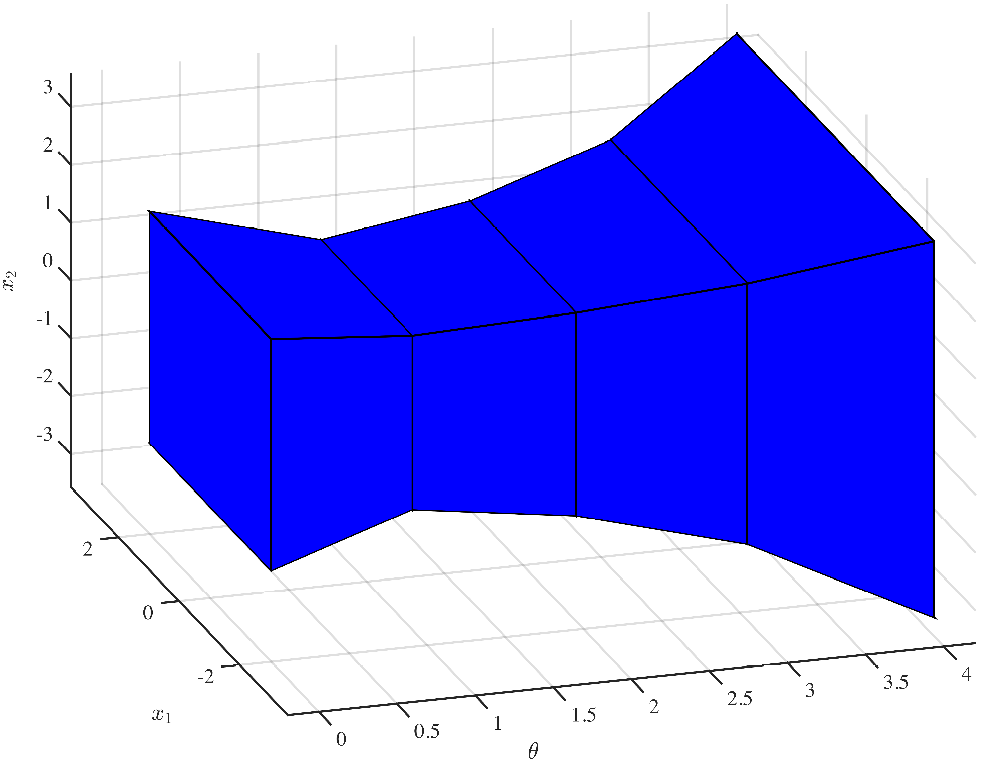
\includegraphics[width=.7\textwidth]{ParametricConvexSet}
\caption[A parametrically convex set.]{The piecewise affine parametric set $\mathcal X(\theta)$ 
defined by $\mathcal X(\theta)\mathrel{\mathop:}=\left\{x:\norm{x}_\infty\leq\max\{-\frac{1}{2}
\theta+2,\frac{1}{4}\theta+\frac{1}{5},\frac{1}{2}\theta+\frac{3}{4},\theta-\frac{3}{4}\}\right\}$ 
for $\theta\in[0,4]$. $\mathcal X(\theta)$ is parametrically convex in~$\theta$.}
\label{fig:parametrically:convex:set}
\end{figure}
%
Notice that Definition~\ref{def:parametric:convexity} does not require convexity of~$\mathcal W(p)$ for all
$p\in X$, we will however only treat maps~$\mathcal W$ for which $\mathcal W(p)$ is convex.
%
In order to compute maximal positive invariant sets for the considered system we need to generalise
the Pontryagin set difference (see e.g.~\cite{blanchini:2007}) to accommodate parametrically convex sets.
%
\begin{defn}[Parametric Pontryagin Difference]\label{def:parametric:pontryagin:difference}
	Let $S\subseteq X$ and let $\mathcal W:X\to\mathcal P(X)$ be a continuous point-to-set map such that
	$\mathcal W(p)$ is convex for all $p\in X$, then the \emph{parametric Pontryagin difference} 
	$S\ominus \mathcal W(S)$ is 
	\begin{equation}\label{eq:definition:parametric:pontryagin:difference}
		S\ominus \mathcal W(S) = \left\{x\in X: \{x\} \oplus \mathcal W(x)\subseteq S\right\},
	\end{equation}
	where $\mathcal W(S)$ denotes the image of $S$ under the map $\mathcal W$. 
\end{defn}
%
At first it may seem sensible to generalise the Pontryagin difference even further and define
%
\begin{equation}\label{eq:extended:parametric:pontryagin:difference}
\begin{split}
	S\ominus \mathcal W(R) &= \{x:\{x\}\oplus \mathcal W(r)\subseteq S\,\forall\, r\in R\}\\
	&=\{x:\{x\}\oplus\bigcup_{r\in R} \mathcal W(r)\subseteq S\}.
\end{split}
\end{equation}
%
However, since $\bigcup_{r\in R} \mathcal W(r)$ may or may not be convex, we can not make any useful
statements about $S\ominus \mathcal W(R)$. 
%
In the case that~$\mathcal W(p)$ is constant, i.e. $\bigcup_{p\in X}\mathcal W(p)=\mathcal W(p)=:C$,
we see that $S\ominus \mathcal W(S)=S\ominus C$ which is the Pontryagin difference for regular sets.
%
For the parametric Pontryagin difference of a convex set and a parametrically convex map we 
have the following result.
%
\begin{thm}\label{thm:convexity:of:pontryagin:difference}
  Let $S\subseteq X$ be a convex set and let $\mathcal W:X\rightarrow\mathcal P(X)$ be a parametrically convex point-to-set
  map such that $\mathcal W(p)$ is convex for all $p\in X$, then $S\ominus \mathcal W(S)$ is convex.
\end{thm}
%
\begin{proof}
To prove the convexity of $ Z :=  S\ominus \mathcal W( S)$ we pick any $z_1,z_2\in Z$, then
by definition of the parametric Pontryagin difference, we have
%
\begin{equation}
	\{z_i\} \oplus \mathcal W(z_i) \subseteq S,\; i=1,2.
\end{equation}
%
To see that $ Z$ is convex we show that line segments between
all possible $z_1$ and $z_2$ are subsets of $ Z$, i.e.~for all $\lambda \in [0,1]$,
\begin{equation}
\begin{aligned}
	\{ \lambda z_1 + (1-&\lambda)z_2
	\}\oplus \mathcal W\left( \lambda z_1 + (1-\lambda)z_2\right)\\
	\subseteq&\left\{ \lambda z_1 + (1-\lambda)z_2
	\right\}\oplus \lambda \mathcal W(z_1) \oplus (1-\lambda)
	\mathcal W(z_2)\\
	\subseteq &\lambda\underbrace{(\{z_1\}\oplus \mathcal W(z_1))}_{\subseteq S}\oplus
	(1-\lambda)\underbrace{(\{z_2\}\oplus \mathcal W(z_2))}_{\subseteq S}\\
	\subseteq& Z
\end{aligned}
\end{equation}
%
where the last inclusion follows from the convexity of $\mathcal S$.
\end{proof}
%
% Now consider a parametrically convex set of the form
% %
% \begin{equation}\label{eq:parametric:polyhedron}
% 	T(s)=\{t:Gt\leq H(s)\},
% \end{equation}
% %
% where each row of $H(s)$ is a convex function in $s\in S$, i.e. each element $H_i(s)$ of 
% $H(s)$ satisfies $H_i(\lambda s_1+(1-\lambda)s_2)\leq \lambda H_i(s_1)+(1-\lambda)H_i(s_2)$ 
% for all $\lambda\in[0,1]$ and $s_1, s_2\in S$. 
% %
% We will use sets for which $H(s)$ is piecewise affine in $s\in S$, i.e. sets
% for which $H_i(s) = \max_k\{f_k s + g_k\}$.
% %
% For sets of this type we have the following result.
% %
% \begin{thm}\label{thm:convex:parametric:set}
%   The point-to-set map $T(s)$ defined by~\eqref{eq:parametric:polyhedron} is parametrically 
%   convex for all $s\in S$ if $H(s)$ is elementwise convex in $s\in S\subseteq X \subset 
%   \mathbb R^n$.
% \end{thm}
% %
% \begin{proof}
% To show that $T(\lambda s_1 + (1-\lambda)s_2)\subseteq \lambda T(s_1) \oplus(1-\lambda)
% T(s_2)$ for all $\lambda \in [0,1]$ and $s_1, s_2\in S$ we note that
% %
% \begin{equation}
% \begin{aligned}
%   T&(\lambda s_1 + (1-\lambda)s_2)\\
%   =& \{t:\; G t \leq H(\lambda s_1 + (1-\lambda)s_2)\}\\
%   \subseteq& \{t:\;Gt\leq\lambda H(s_1)+(1-\lambda) H(s_2)\}\\
%   =&\{t:\;Gt\leq\lambda H(s_1)\}\oplus\{t:\;Gt\leq(1-\lambda)H(s_2)\}\\
%   =&\lambda T(s_1)\oplus(1-\lambda) T(s_2).
%   \end{aligned}
% \end{equation}
% %
% \end{proof} 
% %
% Notice that rays and vertices of $T(s)$ as defined in~\eqref{eq:parametric:polyhedron} will
% be linear combinations of $H_i(s)$, this implies that for piecewise affine $H(s)$ rays
% and vertices $t_k(s)$ will themselves be piecewise affine in $s\in S$, we will exploit
% this fact later on.
%
%
In the following we derive a property for piecewise affine parametric set-valued maps that will
allow convenient computation, namely that it is sufficient to check the number of vertices of 
instances $\mathcal W(p)$ on the boundaries of the parameter space to guarantee the parametric convexity.
%
The statement is summarised in Corollary~\ref{thm:p:convexity:PWA:set:constant:num:verts} in this section.
%
First we introduce the \emph{graph} of $\mathcal W$
%
\[
	\mathscr G(\mathcal W) = \{(p,x) \in\mathbb R^{d+n}: x\in\mathcal W(p)\},
\]
%
its \emph{interior}
%
\[
	\text{int}(\mathscr G(\mathcal W)) = \{(p,x) \in\mathbb R^{d+n}: \forall d\in\mathbb R^n\;\exists 
	\epsilon>0 : x+\epsilon d\in \mathcal W(p)\}
\]
%
and its \emph{boundary}
\[
	\partial \mathscr G(\mathcal W) = \mathscr G(\mathcal W)\setminus \textup{int}(\mathscr G(\mathcal W)).
\]
%
We define the \emph{extended normal cone} as
%
\[
	\mathcal N\mathcal W(p,x) = \{d\in\mathbb R^n: x+\epsilon d \not\in \mathcal W(p)\; \forall \epsilon>0\}
\]
for all $(p,x)\in\partial\mathscr G(\mathcal W)$.
%
\begin{rem}
%
Notice that we define the extended normal cone without an inner product. 
%
The way it is defined here, the conventional normal cone (e.g.~\cite{Boyd:04}) for a convex set $\mathcal C$
%
\[
	N_{\mathcal C}(x) = \{y: \langle y,x-z\rangle\geq0\;\forall z\in\mathcal C\}
\]
%
is be contained in the extended normal cone
%
\[
	\mathcal N_{\mathcal C}(x) = \{y:\exists\epsilon>0\;x+\epsilon y\not\in\mathcal C\}.
\]
%
Furthermore, we have that $\langle d, y\rangle\geq0$ for all $d\in\mathcal N_{\mathcal C}(x), y\in N_{\mathcal C}(x)$.
%
\end{rem}
%
\begin{rem}
%
Notice further that all definitions above are defined relatively for the \emph{set variable} $x$ rather than for graph
variable $(p,x)$.
%
\end{rem}
%
We state the central theorem to connect parametric convexity of a set valued map $\mathcal W$ with properties of its graph
$\mathscr G(\mathcal W)$.
%
\begin{thm}\label{thm:p:convexity:graph}
The map $\mathcal W$ is parametrically convex iff for all $(p_1,x_1),(p_2,x_2)\in\partial\mathscr G(\mathcal W)$
with $\mathcal N\mathcal W(p_1,x_1)\cap\mathcal N\mathcal W(p_2,x_2)\neq\emptyset$ and $p_1\neq p_2$ 
%
\begin{equation}\label{eq:graph:def:p:convexity}
\lambda (p_1,x_1) + (1-\lambda) (p_2,x_2) \not\in\textup{int} (\mathscr G(\mathcal W))
\end{equation}
%
holds for all $\lambda\in(0,1)$.
%
\end{thm}
%
\begin{proof}
%
Assume~\eqref{eq:graph:def:p:convexity} holds for $(p_1,x_1),(p_2,x_2)\in\partial\mathscr G(\mathcal W)$.
%
Then the Minkowski functional (see e.g.~\cite{Rudin:91}) yields $\mu(\mathcal W(\lambda p_1 + (1-\lambda)p_2),
\lambda x_1+(1-\lambda)x_2)\geq1$,
i.e. all interpolation points lie either on the boundary or outside the set $\mathcal W(\lambda p_1+(1-\lambda)p_2)$
therefore the set of all possible interpolation points 
%
\[
	\lambda \mathcal W(p_1)\oplus (1-\lambda)\mathcal W(p_2) = \{x:x=\lambda x_1 + (1-\lambda) x_2 \wedge x_1\in\mathcal 
	W(p_1) \wedge x_2\in\mathcal W(p_2)\}
\]
%
contains the set $\mathcal W(\lambda p_1 + (1-\lambda)p_2)$.
%
Now assume $\mathcal W$ is parametrically convex but~\eqref{eq:graph:def:p:convexity} is not satisfied for 
some $(p_1,x_1),(p_2,x_2)\in\partial\mathscr G(\mathcal W)$ with $\mathcal N\mathcal W(p_1,x_1)\cap\mathcal 
N\mathcal W(p_2,x_2)\neq\emptyset$, i.e. $\lambda x_1 + (1-\lambda)x_2\in\text{int}(\mathcal W(\lambda p_1 + 
(1-\lambda)p_2)$.
%
This implies that a full dimensional ball $B_\epsilon(x ) = \{y:\| 
x-y\|<\epsilon\}$
is contained in $\mathcal W(\lambda p_1 + (1-\lambda)p_2)$, i.e. $B_\epsilon(\lambda x_1 + (1-\lambda)x_2 )\subset
\mathcal W(\lambda p_1 + (1-\lambda)p_2)$ for some $\epsilon>0$.
%
Since $\mathcal N\mathcal W(p_1,x_1)\cap\mathcal N\mathcal W(p_2,x_2)\neq\emptyset$, there exist directions 
$d\in\mathcal N\mathcal W(p_1,x_1)\cap\mathcal N\mathcal W(p_2,x_2)$ which can not be represented as $d=\lambda d_1+
(1-\lambda)d_2$ with $x_1 + \epsilon d_1\in\mathcal W(p_1)$ and $x_2  + \epsilon d_2\in\mathcal W(p_2)$, however since $B_\epsilon$ is full dimensional
all directions exist, $x+\epsilon d\in\mathcal W(\lambda p_1 + (1-\lambda)p_2)$.
%
Hence, $\mathcal W$ can not be parametrically convex.
\end{proof}

\begin{rem}
Notice that condition~\eqref{eq:graph:def:p:convexity} is a non-convexity condition on the graph $\mathscr G(\mathcal W)$.
%
If $\mathscr G(\mathcal W)$ is strictly convex anywhere~\eqref{eq:graph:def:p:convexity} is violated and 
$\mathcal W$ can not be parametrically convex.
\end{rem}
%
\begin{rem}
%
Furthermore notice that the condition on the extended normal cones is only a restriction on the choice of 
$(p,x)$.
%
It is to avoid choices such that the entire line between $(p_1,x_1)$ and $(p_2,x_2)$ is contained in the interior
of the graph by convexity of $\mathcal W(p_i)$.
%
\end{rem}
%
\begin{figure}
\centering 
\begin{lpic}{pConvexSetsAbstract}
\lbl{74,16;$p$}
\lbl{52,20,90;$\mathcal W(p_2)$}
\lbl{10,20,90;$\mathcal W(p_1)$}
\lbl[bl]{17,35,45;$\mathcal N\mathcal W(p_1,x_1)$}
\lbl[bl]{58,37,45;$\mathcal N\mathcal W(p_2,x_2)$}
\lbl[bl]{62,17,45;$\textup{int}(\mathscr{G}(\mathcal W))$}
\lbl[l]{77,4;$\partial \mathscr{G}(\mathcal W)$}
\end{lpic}
\caption[Example p-convex set]{Illustration of the concepts for a scalar parametrically convex map in one-dimension.}
\end{figure}
%
\begin{korr}
%
Let $\mathcal W(p):=\{x\in\mathbb R^n: r(p,x)\leq0\}$ define a set-valued map with a continuous function 
$r: \mathbb R^d \times\mathbb R^n \rightarrow \mathbb R,(p,x)\mapsto r(p,x)$, then $\mathcal W$ is parametrically
convex iff the function $r$ is concave in $p\in\mathbb R^d$ and convex in $x\in\mathbb R^n$.
%
\end{korr}
%
\begin{proof}
The convexity in $x\in\mathbb R^n$ is required to satisfy the requirement that $\mathcal W(p)$ is convex
for all fixed values of $p\in\mathbb R^d$. 
%
Assume that for some region $\Omega\subset\mathbb R^d$ the function $r(\cdot,x)$ is non-concave (i.e. 
strictly convex), any convex subset $\mathcal C\subseteq\Omega$ will hence be such that $\mathscr 
G(\mathcal W)\vert_{\mathcal C}$ is a convex set.
%
In particular all lines between all $(p_1,x_1),(p_2,x_2)\in \partial\mathscr G(\mathcal W)\vert_{\mathcal C}$ will satisfy
$\lambda (p_1,x_1) + (1-\lambda) (p_2,x_2) \in\textup{int} (\mathscr G(\mathcal W))\vert_{\mathcal C}$ since
$\mathscr G(\mathcal W)\vert_{\mathcal C}$ is strictly convex in $p$.
%
This implies that $r(\cdot,x)$ can not be non-concave in any non-trivial set $\Omega\subseteq\mathbb R^d$ and still
be parametrically convex.
\end{proof}
%
\begin{korr}\label{thm:polytopic:set:not:p:convex}
The polytopic parametric set valued map $\mathcal W(p):=\{x: a_i x + b_i p\leq c_i \forall i\leq m\}$ is not parametrically convex for 
any non-trivial matrix $B$.
\end{korr}
%
\begin{proof}
The graph $\mathscr G(\mathcal W)$ is given by
%
\begin{equation*}
	\mathscr G(\mathcal W) = \{(p,x):a_i x + b_i p\leq c_i \forall i\leq m\}
\end{equation*}
%
and hence is a convex set and violates Theorem~\ref{thm:p:convexity:graph}.
\end{proof}
%
We now can prove the following central corollary.
%
\begin{korr}\label{thm:p:convexity:PWA:set:constant:num:verts}
The piecewise affine polytopic parametric set valued map 
%
\begin{equation}\label{eq:definition:PWA:polytopic:set:general}
	\mathcal W(p) := \left\{x: a_i x \leq \max_{k\leq l}\{b_{i,k} + C_{i,k}p\},i\leq m\right\}
\end{equation}
%
is parametrically convex iff the number of vertices $v_i(p)$ and rays $u_i(p)$ is constant.
\end{korr}
%
\begin{proof}
For clarity this proof is divided in 3 parts:
\begin{enumerate}
\item Notice that $h_i(p) = \max_{k\leq l} \{b_{i,k} + C_{i,k}p\}$ is a multi-parametric linear program (mpLP),
its solution is a piecewise affine function $h_i(p) = b_{i,k^\ast_i} + C_{i,k^\ast_i}p$ where $k^\ast_i(p)$ is constant
inside a polytopic complex, see e.g.~\cite{spjotvold:2005}.
%
That means that there exists a finite partitioning $\mathbb R^d = \bigcup_{i\leq t} \mathcal P_i$ with convex polyhedra 
$\mathcal P_i$ such that ${\bf{k}}^\ast\vert_{\mathcal P_i} = (k_1^\ast,\dots,k_m^\ast) = const$.
%
A standard degeneracy assumption is that in neighbouring partitions ${\bf{k}}^\ast\vert_{\mathcal P_i}$ and 
${\bf{k}}^\ast\vert_{\mathcal P_j}$ differ in exactly one element.
%
This partitioning implies that the graph $\mathscr G(\mathcal W)$ is given as a finite union of polyhedra
%
\begin{equation*}
	\mathscr G(\mathcal W) = \bigcup_{j\leq t} \left\{x: a_i x \leq b_{i,k_i^\ast} + C_{i,k_i^\ast}p,i\leq m
	\right\}\bigr\vert_{\mathcal P_j}
\end{equation*}
%
But this implies that if the number of vertices or rays changes in any partition $\mathcal P_i$ then $\mathscr
G(\mathcal W)\vert_{\mathcal P_i}$ is a strictly convex polytope and theorem~\ref{thm:polytopic:set:not:p:convex} applies.
%
\item Our attention hence is concentrated to the boundaries of the partitions $\mathcal P_i$.
%
These are the points $\mathcal P_i \cap \mathcal P_j$ where some mpLP changes its solution, i.e. 
$b_{i,k_{i_1}^\ast} + C_{i,k_{i_1}^\ast} p = b_{i,k_{i_2}^\ast} + C_{i,k_{i_2}^\ast} p$.
%
Notice that a vertex $v_i(p)$ is given by \emph{active} and \emph{inactive} inequalities, i.e. $\mathcal A_i(p)$ and
$\mathcal I_i(p) = \{1,\dots,m\}\setminus\mathcal A_i(p)$ respectively.
%
\begin{equation*}\begin{split}
	a_j v_i(p) &= b_{j,k_j^\ast} + C_{j,k_j^\ast} p \quad\forall j\in\mathcal A_i(p)\\
	a_j v_i(p) &< b_{j,k_j^\ast} + C_{j,k_j^\ast} p \quad\forall j\in\mathcal I_i(p)
\end{split}\end{equation*}
%
In order for the number of vertices to change, there must be a hyperplane $fp=g$, such that the number of vertices for $fp<g$ is 
$N$ and for $fp>g$ is at least $N+1$.
%
It follows from the previous discussion that $\{p:fp=g\} = \textup{aff}\{\mathcal P_i\cap\mathcal P_j\}$ for some $i\neq j$.
%
For vertices $v_i(p)$ and $v_j(p)$ to merge the index sets $\mathcal A_i(p)$ and $\mathcal A_j(p)$ have to differ in only one 
element, i.e. $\mathcal A_i(p) = \mathcal J\cup \{s\}$ and $\mathcal A_j(p) = \mathcal J\cup\{u\}$ for $fp>g$.
%
Furthermore, for $p$ with $fp\leq g$ we have $v_i(p)=v_j(p)$, this implies $\mathcal A_i(p) = \mathcal A_j(p)$.
%
Since only one alteration of the active index set is considered (due to generic assumptions), the active set $\mathcal A_i(p) = \mathcal A_j(p)
= \mathcal J \cup \{s,u\}$.
%
Hence on the hyperplane $fp=g$ both, the maximising index ${\bf{k}}^\ast(p)$ and the active index sets $\mathcal A_i(p)$ 
and $\mathcal A_j(p)$ change, which is degenerate.
%
\item In order for the degenerate graph $\mathscr G(W)$ to be parametrically convex the overdetermined vertex $v_i(p)=v_j(p)$
have to be identical, in particular their dependence on $p$ has to be identical.
%
This can be expressed with the implicit function theorem:
%
\begin{equation*}\begin{split}
	\frac{d}{dp}\left(	A_{\mathcal J\cup \{s\}} v_i(p) - b_{\mathcal J\cup \{s\}} - C_{\mathcal J\cup \{s\},{\bf{k}}^\ast} p\right) &= 0\\
	\frac{d}{dp}\left(	A_{\mathcal J\cup \{u\}} v_i(p) - b_{\mathcal J\cup \{u\}} - C_{\mathcal J\cup \{u\},{\bf{k}}^\ast} p\right) &= 0
\end{split}\end{equation*}
%
which leads to 
%
\begin{equation*}\begin{split}
	A_{\mathcal J\cup \{s\}} \frac{dv_i}{dp} &= C_{\mathcal J\cup \{s\},{\bf{k}}^\ast}\\
	A_{\mathcal J\cup \{u\}} \frac{dv_i}{dp} &= C_{\mathcal J\cup \{u\},{\bf{k}}^\ast}
\end{split}\end{equation*}
%
since we can assume that the inequalities are non-redundant for some right hand side, we obtain that 
%
\begin{equation}\label{eq:derivative:condition:on:index:sets}
	\frac{dv_i}{dp} = A_{\mathcal J\cup \{s\}}^{-1}C_{\mathcal J\cup \{s\},{\bf{k}}^\ast} = 
	A_{\mathcal J\cup \{u\}}^{-1}C_{\mathcal J\cup \{u\},{\bf{k}}^\ast}
\end{equation}
%
has to hold for the degenerate graph to remain parametrically convex.
%
Notice that~\eqref{eq:derivative:condition:on:index:sets} is again a degenerate condition, since arbitrarily small perturbations
will produce different behaviour.
\end{enumerate}
\end{proof}
%
\begin{rem}
Corollary~\ref{thm:p:convexity:PWA:set:constant:num:verts} is essential for numerical examples, as it can be reformulated to:
%
The set valued map defined by~\eqref{eq:definition:PWA:polytopic:set:general} is parametrically convex iff it has a constant 
number of vertices throughout the parameter space~$X$.
%
\\[1em]
%
Since the map is continuous it is sufficient to verify this at the vertices of the parameter space.
%
\end{rem}
%
To illustrate the effects of perturbations to a degenerate piecewise affine map, consider the following low dimensional 
examples:
%
\begin{quote}
Let $\mathcal W_i(p)$ be defined by
%
\begin{equation*}\begin{split}
	\mathcal W_1(p) = \left\{x : \left(\begin{array}{cc}
	1&1\\
	-1&1\\
	0&1\\
	0&-1 
	\end{array}\right)x \leq \left(\begin{array}{c}
	\max\{1+p,\frac{1}{2}+2p\} \\
	\max\{1+p,\frac{1}{2}+2p\} \\
	\frac{1}{2}+2p \\
	1
	\end{array}\right)
	\right\}\\
%
	\mathcal W_2(p) = \left\{x : \left(\begin{array}{cc}
	1&1\\
	-1&1\\
	0&1\\
	0&-1 
	\end{array}\right)x \leq \left(\begin{array}{c}
	\max\{1+p,\frac{1}{2}+(2+\epsilon)p\} \\
	\max\{1+p,\frac{1}{2}+2p\} \\
	\frac{1}{2}+2p \\
	1
	\end{array}\right)
	\right\}\\
%
	\mathcal W_3(p) = \left\{x : \left(\begin{array}{cc}
	1&1\\
	-1&1\\
	0&1\\
	0&-1 
	\end{array}\right)x \leq \left(\begin{array}{c}
	\max\{1+p,\frac{1}{2}+\epsilon+2p\} \\
	\max\{1+p,\frac{1}{2}+2p\} \\
	\frac{1}{2}+2p \\
	1
	\end{array}\right)
	\right\}
	\end{split}
\end{equation*}
%
%
\begin{figure}
\begin{center}
\subfigure[$\mathcal W_1(p)$]{\includegraphics[width=.45\textwidth]{pConvDegenerateSet}}
\subfigure[$\mathcal W_2(p)$]{\includegraphics[width=.45\textwidth]{pConvPertInLinTerm}}\\
\subfigure[$\mathcal W_3(p)$]{\includegraphics[width=.45\textwidth]{pConvPertInConstantTerm}}
\end{center}
\caption[Degenerate PWA p-convex sets]{For $\mathcal W_1(p)$ the right hand side was chosen in order 
to satisfy~\eqref{eq:derivative:condition:on:index:sets} 
and for the graph to be degenerate. For both $\mathcal W_{2,3}(p)$ there is no drop in number of vertices for different 
$p\in[-1,\infty),\epsilon=10^{-1}$.}
\label{fig:degenerate:PWA:set:and:comparison}
\end{figure}
%
See figure~\ref{fig:degenerate:PWA:set:and:comparison} for an illustration.
\end{quote}
%
%
%
%
%
\section{Example}\label{sec:example:linearisation:error:as:state:dependent:constraint}
In this section we derive a disturbance set that is of the form~\eqref{eq:derivative:condition:on:index:sets}
with a piecewise affine right hand side~$H(s)$. 
%
Consider a discrete time nonlinear system of the form
%
\begin{equation}
	x^+ = f(x,u)
\end{equation}
%
with $x_e=f(x_e,u_e)$ as an equilibrium point. 
%
Close to the equilibrium point the dynamics can be approximated by ${\tilde x}^+ = A \tilde x 
+ B\tilde u$ with $\tilde x = x-x_e$ and $\tilde u = u - u_e$ and the linearisation matrices
$A = \frac{\partial f}{\partial x}\vert_{(x_e,u_e)}$ and $B = \frac{\partial f}{\partial u}
\vert_{(x_e,u_e)}$.
%
We want to describe the dynamics of the nonlinear system with those of its linearisation considering
an additive disturbance. 
%
I.e. we want that for all $x\in X_c$ and $u\in U_c$ there exists a realisation 
$v\in V(x,u)$ such that the identity $f(x,u)=Ax + B u + v$ holds. 
%
In order to derive a parametrised set $V(x,u)$ such that the desired identity holds we use
the mean value theorem (see e.g.~\cite{Apostol:1974}):
%
\begin{thm}[Mean Value Theorem]\label{thm:mean:value:theorem}
Let $g : \mathcal X \rightarrow\mathbb R^m$ be continuously
differentiable, $\mathcal X\subset\mathbb R^n$ be open,
and $x \in\mathcal X$, $h \in\mathbb R^n$ be such that 
$x + th \in\mathcal X$ for all $t\in [0 ,1]$. Then
\begin{equation}
	g(x+h) = g(x) + \left(\int_0^1 \frac{\partial g}{\partial x}(x+th)dt\right)\cdot h.
\end{equation}
\end{thm}
%
We can use this to state
%
\begin{equation}
\begin{split}
	f(x_e+x,u_e+u)-A(x_e+x)-B(u_e+u) = \underbrace{f(x_e,u_e) - A x_e - B u_e}_{=0} \\
	+ \int_0^1\left(\frac{\partial f}{\partial x}(x_e+tx,u_e+tu) \cdot x + 
	\frac{\partial f}{\partial u}(x_e+tx,u_e+tu) \cdot u \right) dt -Ax-Bu\\
	= \underbrace{\left(\int_0^1 \frac{\partial f}{\partial x}(x_e+tx,u_e+tu) dt - A\right)}_{H^x} x + 
	\underbrace{\left(\int_0^1 \frac{\partial f}{\partial u}(x_e+tx,u_e+tu) - B \right)}_{H^u} u.
\end{split}
\end{equation}
%
This means that for any given $(x,u)\in X\times U$ we can compute an additive disturbance $v=H^x x + H^u u$
such that $f(x_e+x,u_e+u)-Ax-Bu = v$.
%
Assume we had all possible $H^x$ and $H^u$ for all $(x,u)\in X\times U$ given, clearly then 
$\min\{H^x x + H^u u\} \leq f(x_e+x,u_e+u)-Ax-Bu \leq \max\{H^x x + H^u u\}$ holds true.
%
For general nonlinear systems there is no way to obtain an analytic solution for $H^x$ and $H^u$,
so instead $K$ samples of $X\times U$ have to be used to obtain a description of 
the disturbance set
%
\begin{equation}\label{eq:derivation:of:PWA:disturbance:set}
\begin{split}
	V^K(x,u) &= \left\{v: \min_{k\leq K}\{H^x_k x + H^u_k u\} \leq v \leq \max_{k\leq K}\{H^x_k x + H^u_k u\} \right\}\\
	&= \left\{v: v \leq \max_{k\leq K}\{H^x_k x + H^u_k u\} \wedge -v \leq \max_{k\leq K}\{-H^x_k x - H^u_k u\} \right\}
\end{split}
\end{equation}
%
Notice that sampling the set $\gimel(x,u) = \left\{v : \min\{H^x x + H^u u\} \leq v \leq \max\{H^x x + H^u u\}\right\}$ 
leads to an inner approximation which is convexified by taking its convex hull.
%
The set $V^K(x,u)$ as defined in~\eqref{eq:derivation:of:PWA:disturbance:set} is of the
type~\eqref{eq:derivative:condition:on:index:sets} with a piecewise linear right hand side. We may
want to add a constant term to accommodate model uncertainties.
%
%
%
%
\section{Maximal Positive Robust Invariant Sets}\label{sec:parametrised:MRPI:set}
In this section we present a way to calculate maximal robust positive invariant sets for
linear discrete time systems under the influence of additive perturbation.
%
We assume the perturbation to be constrained in sets which are piecewise affine in
the state, i.e.
%
\begin{equation}\label{eq:definition:PWA:uncertainty}
v\in \mathcal V(x) = \left\{v: Gv\leq\max_k\{H_k^x x + h_k\}\right\}.
\end{equation}
%
The definition of the maximal robust positive invariant set in this scenario is given as
the largest set satisfying
%
\begin{equation}\label{eq:MRPI:state:dependent:disturbance}
	\mathcal X^\infty = \left\{x: \Psi x + v \in\mathcal X^\infty\,\forall\, v\in\mathcal V(x)\right\},
\end{equation}
%
largest in the sense that it includes all smaller ones.
%
The implicit definition of~\eqref{eq:MRPI:state:dependent:disturbance} suggests a recursive 
computation of $\mathcal X^\infty$.
%
We assume system dependent state constraints $\mathscr X\subseteq\mathbb R^n$ are given,
we furthermore assume that $\mathscr X$ is polyhedral and contained in a band.
%
\begin{defn}[Band Property]
We say that a set $X\subseteq\mathbb R^d$ possesses the band property if there exists a 
matrix~$\Gamma\in\mathbb R^{p\times d}$ such that $X\subseteq B = \{x:\Gamma x\leq {\bf{1}}\wedge
-\Gamma x\leq{\bf{1}}\}.$
\end{defn}
%
That is, we assume that $\mathscr X= \{x:\Lambda_i x \leq \lambda_i \forall\, i\leq m\}\subseteq\{x:\Gamma x\leq{\bf{1}}\wedge
-\Gamma x\leq{\bf{1}}\}=:\mathscr B$.
%
In the following we discuss how to apply the principle of the Kolmanovsky and Gilbert 
algorithm\footnote{The concept was first introduced for 
unperturbed systems in 1991 by Gilbert and Tan~\cite{Gilbert:1991}, therefore all its derivatives 
are also referred to as the \emph{Gilbert and Tan algorithms}.} 
presented in~\cite{Kolmanovsky:1995}.
%
The algorithm is a recursive iteration: Starting from $\mathscr X$ we 'cut off' all such stated 
for which the successor state would violate~\eqref{eq:MRPI:state:dependent:disturbance}, i.e.
in the $n^\text{th}$~iteration we introduce constraints which enforce that the trajectories
of all points in the set would remain in the set for $n$~time steps.
%
This means that in the first iteration we enforce that for all points in the iterate the 
successor state is contained in the initial set $x^+\in X_0 = \mathscr X$:
%
\begin{equation}\label{eq:PWA:disturbance:first:iterate}
\begin{split}
	X_1 &= \{x: \Psi x + v\in X_0 \forall v\in\mathcal V(x)\}\\
	&=\{x:\Lambda_i(\Psi x +v)\leq \lambda_i \forall\,i\leq m_0\}\\
	&=\left\{x:\Lambda_i\Psi x + 
	\underbrace{\left\{\begin{array}{rl}\max& \Lambda_i v\\ 
	\text{s.t.}& v\in\mathcal V(x)
	\end{array}\right\}}_{\gamma_{1,i}^\ast(x)} \leq \lambda_i \forall\,i\leq m_0\right\}
\end{split}
\end{equation}
This requires the solution $m_0$ multi-parametric linear programs\footnote{Multi-parametric 
linear programs have been introduced as optimisation problems
in the late 1958 by~\cite{Courtillot:1958}. Various ways to solve mpLPs have been proposed.}
(mpLPs) in order to obtain~$v_{1,i}^\ast(x)$.
%
However, the solution of multi-parametric linear programs will be given by vertices 
of the constraint set, i.e. $\gamma_{1,i}^\ast(x)=\Lambda_i v_{k^\ast}(x)$ where $v_{k^\ast}(x)$
is the optimising vertex.
%
Recall that since $\mathcal V(x)$ is piecewise affine in $x$ its vertices will also be piecewise 
affine in $x$, i.e. there exists a representation $v_k(x)=\max_{l\leq K_k}\{W_l^k x + w_l^k\}$.
%
Notice that we do not need to solve all mpLP in order to compute $X_1$, adding all available
$W_l,w_l$ produces the desired set without solving $m_0$ mpLP:
%
\begin{equation}\label{eq:derivation:of:row:reduction:instead:of:mpLP}
\begin{split}
	X_1 &= \{x: \Lambda_i\Psi x + \gamma_{1,i}^\ast(x)\leq\lambda_i \,\forall i\leq m_0 \}\\
	&= \left\{x: \Lambda_i\Psi x + \max_l\{\Lambda_i (W_l^{k^\ast} x + w_l^{k^\ast}) \} \leq \lambda_i\, 
	\forall i\leq m_0 \right\} \\
	&= \left\{x: (\Lambda_i\Psi + \Lambda_i W_l^{k^\ast}) x \leq \lambda_i-\Lambda_i w_l^{k^\ast}\,
	\forall i\leq m_0, l\leq K_k  \right\} \\
	&= \left\{x: (\Lambda_i\Psi + \Lambda_i W_l^k) x \leq \lambda_i - \Lambda_i w_l^k\,
	\forall i\leq m_0, l\leq K_k, k\leq \kappa \right\}.
\end{split}
\end{equation}
%
The equalities~\eqref{eq:derivation:of:row:reduction:instead:of:mpLP} hold since only the 
inequalities which define~$\gamma_{1,i}^\ast(x)$ will define the set~$X_1$, i.e. we avoid
solving mpLP by introducing redundant inequalities, instead of $m_0$ supporting hyperplanes
we describe the set by $m_1 = m_0\cdot \kappa\cdot \prod_{k\leq \kappa} K_k$ hyperplanes with
a large number of them being redundant, here~$\kappa$ denotes maximal the number of vertices 
of~$\mathcal V(x),\,x\in\mathscr X$.
%
This seems to be a poor trade off, however, we can use inequality reduction algorithms at any
point of the iteration and reduce the number of hyperplanes~$m_1$ in the representation of~$X_1$.

The next set iterate~$X_2$ is then defined by
%
\begin{equation}
	\begin{split}
	X_2 &= \left\{x: \Psi (\Psi x + v) + \tilde v\in X_0\,\forall v,\tilde v\in\mathcal V(x) \right\}\\
	&= \{x\in X_1 : \Psi x + v \in X_1\,\forall v\in\mathcal V(x)\}\\
	&= X_1 \cap \{x: \Psi x + v \in X_1\,\forall v\in\mathcal V(x)\},
	\end{split}
\end{equation}
%
so that successive set iterates can be defined recursively.
%
The general iterate is given by:
%
\begin{equation}\label{eq:general:MRPI:iteration}
	X_{k+1} = X_k \cap \{x:\Psi x + v\in X_k\, \forall v\in\mathcal V(x)\}
\end{equation}
%
It is obvious that by its definition $X_{k+1}\subseteq X_k$, once $X_k\subseteq X_{k+1}$ holds
the iteration~\eqref{eq:general:MRPI:iteration} terminates.
%
$X_k\subseteq X_{k+1}$ implies that all $x\in X_k$ also satisfy $x\in X_{k+1}$, however
$X_{k+1}$ is defined as points to which the successor state is contained in $X_k$, therefore
$X_{k+1} = \mathcal X^\infty$. 

In the remainder of this section we will prove that the described algorithm terminates 
in a finite number of iterations.
%
Notice that the set iterates defined by~\eqref{eq:general:MRPI:iteration} can be formally
be defined by
%
\begin{equation}
	X_{k+1} = X_k \cap \{x: \Lambda_i\Psi^k x + \sum_{l=1}^{k-1} \gamma_{l,i}^\ast(x)\leq\lambda_i\,
	\forall i\leq m_0\},
\end{equation}
%
where
%
\begin{equation}\begin{split}
	\gamma_{l,i}^\ast(x) &= \max_j \Lambda_i\Psi^{l-1} v_j(x) \\
	&= \begin{array}{rl} \max_v &\Lambda_i\Psi^{l-1} v\\
		\text{s.t.} & v\in\mathcal V(x)\end{array} \\
	&= \begin{array}{rl} \max_{\tilde v} &\Lambda_i \tilde v\\
		\text{s.t.} & \tilde v\in \Psi^{l-1}\mathcal V(x) \end{array}.
\end{split}\end{equation}
%
So that~\eqref{eq:general:MRPI:iteration} becomes
%
\begin{align}
	X_{k+1} &= X_k \cap \left( \Psi^{-k-1} X_0\, \underset{1\leq i\leq k}{\bigominus} 
	\Psi^{i-1}\mathcal V(X_k) \right)\nonumber \\
	&=\bigcap_{l\leq k+1}\left(\Psi^{-l} X_0 \underset{1\leq i\leq l-1}{\bigominus} 
	\Psi^{i}\mathcal V(X_{l-1}) \right). \label{eq:MRPI:recursion:closed:form}
\end{align}
%
The structure of~\eqref{eq:MRPI:recursion:closed:form} is of central importance for the proof
of finite determinability of~$\mathcal X^\infty$.
%
The first statement we can prove is the following:
%
\begin{thm}\label{thm:band:implies:compactness}
Let the system constraints be contained in a band~$\mathscr X\subseteq \mathscr B 
=\{x: \Gamma x\leq{\bf{1}}\wedge -\Gamma x\leq{\bf{1}}\}$, let $0\in\mathcal V(x)$ for all $x\in\mathscr X$ 
and let the pair $(\Psi,\Gamma)$ be observable, then there exists a natural number $N\leq n$ such 
that~$X_N$ is compact.
\end{thm}
%
\begin{proof}
First recall the fact that $\mathcal A\ominus \mathcal B\subseteq\mathcal A$ if $0\in\mathcal B$,
see e.g.~\cite{blanchini:2007}, this fact extends to the parametric Pontryagin difference.
%
Therefore we have
%
\begin{equation}
	X_k= \bigcap_{l\leq k}\left(\Psi^{-l} X_0 \underset{1\leq i\leq l-1}{\bigominus} 
	\Psi^{i}\mathcal V(X_{l-1}) \right) \subseteq \bigcap_{l\leq k} \Psi^{-l} X_0
	= \bigcap_{l\leq k} \Psi^{-l}\mathscr X \subseteq \bigcap_{l\leq k} \Psi^{-l} \mathscr B.
\end{equation}
%
Note that observability of $(\Psi,\Gamma)$ is equivalent to the observability matrix
\[
	\Omega_o = \left(\begin{array}{c}
	\Gamma \\ \Gamma \Psi \\ \vdots \\ \Gamma \Psi^{n-1}
	\end{array}\right)
\]
%
has full rank.
%
This is equivalent to the null space of $\Omega_o$ being trivial, i.e.~$\ker\Omega_o=\{0\}$,
which implies that~$\{x: \Omega_o x \leq {\bf{1}} \wedge -\Omega_o x \leq {\bf{1}}\}$ is bounded.
%
Note further that
\begin{equation}
	X_n \subseteq \bigcap_{k\leq n} \Psi^{-k}\mathscr B = \left\{x:\underset{k\leq n}{\bigwedge} 
	\pm \Gamma\Psi^{k}x\leq{\bf{1}} \right\} =\{x: \Omega_o x \leq {\bf{1}}\wedge -\Omega_o x\leq{\bf{1}} \}.
\end{equation}
%
Therefore we conclude that $X_n$ is contained in a compact set, hence is itself bounded.
%
The case that~$N<n$ is possible for matrices $\Gamma$ with $\text{rank}(\Gamma)>1$.
\end{proof}
%
We can use Lemma~\ref{thm:band:implies:compactness} to prove the following statement:
%
\begin{thm}[\footnote{
	The earliest proof of finite determinability of the proposed algorithm was published 
	in~\cite[Theorem 4.2]{Kolmanovsky:1995}, the assumptions made for Lemma~\ref{thm:band:implies:compactness}
	and~\ref{thm:finite:terminability:MRPI:algorithm} coincide for the case of constant disturbance sets.
	%
	The formulation chosen here is more explicit than the one stated in~\cite{Kolmanovsky:1995}, since
	all conditions are on data available before initialising the algorithm.
	}]
\label{thm:finite:terminability:MRPI:algorithm}
Let the assumptions for Lemma~\ref{thm:band:implies:compactness} hold, let furthermore
$x^+=\Psi x$ be asymptotically stable and let $\mathcal V(x)$ be bounded for all $x\in\mathscr X$, 
then iteration~\eqref{eq:general:MRPI:iteration} with $X_0=\mathscr X$ terminates in a finite 
number of number of steps.
\end{thm}
%
\begin{proof}
Using~\eqref{eq:general:MRPI:iteration} we can easily see that if for some $k>0$
the set iterate $X_k$ is empty that implies that $X_k=\mathcal X^\infty = \emptyset$,
in this trivial case we can easily see that the algorithm terminates after $k$ iterations.
%
For the remainder of this proof we assume that all set iterates are non-empty.

Let $\rho$ denote the spectral radius of $\Psi$, since $\Psi$ is asymptotically
stable we have $\rho<1$.
%
Let $r_1$ be the radius of the largest ball contained in $X_0$ i.e. $\mathcal E(r_1)\subseteq X_0$ 
and let $r_2$ be the radius of smallest ball containing $V(x)$ for all $x\in X_0$.
%
Recall that $X_k = \bigcap_{l\leq k} D_l$, where $D_k$ is defined by
%
\begin{equation}
	D_l = \underbrace{\Psi^{-l} X_0}_{\mathcal S_1} \ominus 
	\underbrace{\left(\bigoplus_{1\leq i\leq l-1} \Psi^{i}\mathcal V(X_{l-1})\right)}_{\mathcal S_2}
\end{equation}
%
We can easily lower bound $\mathcal S_1$ by using $r_1$: $\mathcal S_1 = \Psi^{-l} X_0 
\supseteq \Psi^{-l}\mathcal E(r_1) \supseteq \mathcal E(\rho^{-l} r_1)$.
%
Recall that $X_l\subseteq X_{l-1}$ and therefore $X_l\subseteq X_0$ for all $l\geq0$.
%
We use this fact to obtain the containment $\mathcal S_2 = \bigoplus_{1\leq i\leq l-1} 
\Psi^{i}\mathcal V(X_{l-1})\subseteq \bigoplus_{1\leq i\leq l-1} \Psi^{i}\mathcal V(X_0)\subseteq
\bigoplus_{1\leq i\leq l-1} \Psi^{i}\mathcal E(r_2)\subseteq\bigoplus_{1\leq i\leq l-1} \mathcal E(\rho^{i} r_2)\subseteq
\mathcal E(\sum_{1\leq i\leq l-1}\rho^i r_2)\subseteq \mathcal E(\frac{1}{1-\rho} r_2)$.
%
In summary we can state that~$D_l$ consists of the exponentially expanding set~$\mathcal S_1$
subtracted by the set~$\mathcal S_2$ which is bounded, therefore~$D_l$ itself expands exponentially,
that is $D_l\supseteq\mathcal E(\rho^{-l} r_1 - \frac{1}{1-\rho} r_2)$.
%
Due to Lemma~\ref{thm:band:implies:compactness} we know that for $N\leq n$ the set iterate~$X_N$ is
bounded, let $r_3$ denote the smallest ball that contains $X_N$.
%
We can conclude that for $l$ such that $X_N\subseteq\mathcal E(r_3)\subseteq\mathcal 
E(\rho^{-l} r_1 - \frac{1}{1-\rho} r_2)\subseteq D_l$ holds the set $D_l$ covers
$X_N$, i.e. intersections with $D_l$ will not change $X_l$.
%
We can therefore give an upper bound on the number of iterations necessary for the algorithm
to terminate, it is given by the smallest integer $M$ such that
\begin{equation}\label{bnd:first:lower:bound:on:iteration:count}
	M\geq \frac{1}{\log(\frac{1}{\rho})}\left(\log\left(r_3+\frac{1}{1-\rho}r_2\right)-\log r_1 \right)
\end{equation}
is satisfied.
\end{proof}
%
Notice that the constants used in~\eqref{bnd:first:lower:bound:on:iteration:count} are not
quite convenient to compute, we can however compute bounds on $r_1,\, r_2$ and $r_3$ using 
singular values.
%
For this let $\bar\sigma(\Gamma)$ and $\underline\sigma(\Gamma)$ denote the maximal and the minimal
singular value of~$\Gamma$ respectively.
%
We know that~$\bar\sigma(\Gamma)\norm{x}\geq\norm{\Gamma x}$ and therefore $\bar\sigma(\Gamma)\norm{x}
\leq \sqrt{n}\Rightarrow \norm{\Gamma x}\leq\norm{\bf{1}}=\sqrt{n}$, that $r_1=\frac{\bar\sigma(\Gamma)}{\sqrt{n}}$
follows form standard result for singular values, see e.g.~\cite{Golub:1996}.
%
We use a similar argument to obtain a bound on $r_3$ before deriving a bound on $r_2$:
%
It is easy to see that the radius of the largest ball containing $X_N$ is given by the maximal
norm of its vertices, i.e. $r_3=\max_{i}\norm{x_i}$ where $x_i$ satisfies $\Omega_{o,\mathscr{A}_i} x_i={\bf{1}}$
and $\Omega_{o,\bar{\mathscr A}_i}x_i<{\bf{1}}$.
%
From this we can deduce that
%
\begin{equation}\begin{split}
	\sqrt{n}=\norm{\bf{1}}=\norm{\Omega_{o,\mathscr{A}_i}x_i}\geq\underline\sigma(\Omega_{o,\mathscr{A}_i})\norm{x_i}
	=\underline\sigma(\Gamma_{\mathscr{A}_i}\cdot \text{diag}(I,\Psi,\dots,\Psi^{n-1}))\norm{x_i}\\
	\geq\underline\sigma(\Gamma_{\mathscr{A}_i})\underline\sigma( \text{diag}(I,\Psi,\dots,\Psi^{n-1}))\norm{x_i}
	\geq\underline\sigma(\Gamma_{\mathscr{A}_i})\underline\sigma(\Psi)^{n-1}\norm{x_i}\\
	\geq\underline\sigma(\Gamma)\underline\sigma(\Psi)^{n-1}\norm{x_i},
\end{split}\end{equation}
%
which implies that we can get the upper bound $r_3\leq\frac{\sqrt{n}}{\underline\sigma(\Gamma)
\underline\sigma(\Psi)^{n-1}}$.
%
In order to obtain an estimate on $r_2$ we follow a similar argumentation:
%
\begin{equation}\begin{split}
	\bar\sigma(H_{k^\ast})\norm{x}+\norm{h_{k^\ast}}=\max_k\{\bar\sigma(H_k)\norm{x}+\norm{h_k}\}\geq
	\norm{\max_k\{H_k x + h_k\}_{\mathscr{A}_i}}\\ 
	=\norm{G_{\mathscr{A}_i}v_i} \geq\underline\sigma(G_{\mathscr A_i})\norm{v_i}
	\geq\underline\sigma(G)\norm{v_i}.
\end{split}\end{equation}
%
Notice that with only the assumptions made in Lemma~\ref{thm:finite:terminability:MRPI:algorithm}
we have no way to bound~$\norm{x}$ in order to obtain an upper bound on~$r_2$,
however, if we assume that~$X_N$ is not empty we can use the bound on~$X_N$, i.e.~$r_3$.
%
This is reasonable since we are interested in the asymptotic behaviour of the set rather than
exact bounds on intermediate iterates, hence $r_2\leq\frac{\bar\sigma(H_{k^\ast})r_3+\norm{h_k}}
{\underline\sigma(G)}$ can be used as an estimate for the asymptotic behaviour of $\mathcal V(x)$
in the iteration.
%
All bounds and estimates on $r_1,\,r_2$ and $r_3$ can be calculated in advance to get an estimate
on how many iterations the described algorithm could require.
%
%
%
%
%
\section[Stage constraints]{Stage constraints for state and input dependent constraints}\label{sec:stage:constraints:state:dependent}
%
In this section we present an algorithm to compute the stage constraints~\eqref{eq:concepts:def:stage:constraints}
a setup with piecewise affine disturbance constraints, i.e. the disturbance set is given by
%
\begin{equation}
	\mathcal V(x,u) = \left\{v: G_i v\leq \max_{k\leq N_i}\{H_{i,k}^x x + H_{i,k}^u + h_{i,k}\}\; 
	i\in\mathcal I_{\mathcal V}\right\}
\end{equation}
%
and $u\in\mathcal U=\{u:Fu\leq{\bf{1}}\}$.
%
The stage constraints are initialised with the polytopic MRPI set $\mathcal X_0=\mathcal X^\infty = 
\{x:\Xi_{i,0} x\leq\xi_{i,0}\;i\in\mathcal I_0\}$ and hence the stage constraints for the penultimate stage~$\mathcal Z_1$
are given by
%
\begin{equation*}\begin{split}
	\mathcal Z_1 &= \{(x,u): Fu\leq{\bf{1}}\wedge \Xi_{i,0}(Ax+Bu + v)\leq\xi_{i,0}\; \forall v\in\mathcal V(x,u), i\in\mathcal I_0\}\\
	&=\left\{(x,u): Fu\leq{\bf{1}}\wedge \Xi_{i,0}A x + \Xi_{i,0} Bu + \max_{v\in\mathcal V(x,u)} \Xi_{i,0}v \leq \xi_{i,0} \;\forall i\in\mathcal I_0
	\right\}\\
	&=\left\{(x,u): Fu\leq{\bf{1}}\wedge \Xi_{i,0}A x + \Xi_{i,0} Bu + \max_{j\in\mathcal I_{\mathcal V}} \Xi_{i,0}v_j(x,u) \leq \xi_{i,0} \;\forall i\in\mathcal I_0
	\right\}\\
	&=\left\{(x,u): Fu\leq{\bf{1}}\wedge \Xi_{i,0}A x + \Xi_{i,0} Bu + \Xi_{i,0}v_{j^\ast}(x,u) \leq \xi_{i,0} \;\forall i\in\mathcal I_0
	\right\}
\end{split}\end{equation*}
%
as in the iteration for the MRPI set~$v_{j^\ast}(x,u)$ does not need to be explicitly determined along each facet.
%
Instead introducing all possible~$v_j(x,u)$ and using an inequality reduction algorithm will produce the desired
result of $\mathcal Z_1 = \{(x,u): E_{i,1}^x x + E_{i,1}^u u\leq e_{i,1};\forall i\in\mathcal J_1\}$,
its projection $\mathcal X_1$ can be obtained by any projection method and is then given by~$\mathcal X_1 = \{x:\Xi_{i,1}x\leq\xi_{i,1}\;\forall i\in\mathcal I_1\}$.
This procedure is repeated recursively for the desired horizon length~$N$.
%
%
%
%
\section{Example}\label{sec:example:parametrised:MRPI:set}
\begin{figure}
\centering
\begin{lpic}{levitatingBall}
\lbl[tr]{25,3; $m g$}
\lbl[br]{25,25; $c\frac{i^2}{y^2}$}
\lbl[bl]{49,17; $y$}
\lbl[bl]{56,55; $i$}
\end{lpic}
\vspace{-2mm}
\caption{Levitating ball system.}
\label{fig:levitating:ball}
\end{figure}
%
%
%
%
In this section we present the calculation of the MRPI set and stage constraints for a linearised simplified model of the magnetic 
levitation system depict in figure~\ref{fig:levitating:ball}. 
%
The system dynamics for the ball are given by $m \ddot y = m g - c\frac{i^2}{y^2}$, where $m,g,c,i$ and $y$ 
denote the mass of the ball, the gravitational constant, a constant factor, the current and the distance 
between the coil and the centre of the ball respectively.
%
For illustration purposes we neglect inductive dynamics and use the current $u=i$ as an input and the position
$y$ and its first derivative $\dot y$ as the states, i.e. $x = (y,\dot y)^T$. 
%
We find that any equilibrium has $\dot{y}=0$ and $u=\sqrt{\frac{gm}{c}} y$ for any positive position $y>0$. 
%
We use the method described in example~\ref{sec:example:linearisation:error:as:state:dependent:constraint}
to obtain a linear system with piecewise affine disturbance modelling the nonlinearites. 
%
Linearising the nonlinear differential equation $\dot x = f(x,u)$ around an equilibrium point $(\hat x, \hat u)$ 
gives the approximate linear model 
%
\begin{equation}
	 \Delta\dot{x} = \underbrace{\left(\begin{array}{cc}
	0 & 1 \\ \frac{2c\hat u^2}{m\hat x_1^3} & 0
	\end{array}\right)}_{\frac{\partial f}{\partial x}(\hat x,\hat
      u)}\Delta x 
+ \underbrace{\left(\begin{array}{c}
	0 \\ - \frac{2c\hat u}{m\hat x_1^2}
	\end{array}\right)}_{\frac{\partial f}{\partial u}(\hat x,\hat
      u)}\Delta u
\end{equation}
%
where $\Delta u = u -\hat{u}$ and $\Delta x \approx x-\hat{x}$.
%
We derive the discrete time dynamics with sampling rate $T_s$ using the Euler formula $x^+=x+T_s f(x,u) =:\tilde f(x,u)$ 
giving
%
\[
\Delta x^+ = A \Delta x + B \Delta u , \quad
\Biggl\{\begin{aligned} A &= I+T_s\frac{\partial f}{\partial  x}(\hat
  x,\hat u) \\
B &= T_s \frac{\partial f}{\partial u}(\hat x,\hat u)
\end{aligned}
\]
%
Although this system has a control input, the algorithm for computing the MRPI set is applicable since we consider 
the closed loop system under linear feedback  $u=Kx$, where $K$ is designed to satisfy a robust Lyapunov condition 
described in Appendix~\ref{app:terminal:controller}, see e.g.~\cite{Boyd:94}.
%
We use the method derived in example~\ref{sec:example:linearisation:error:as:state:dependent:constraint} to 
obtain piecewise affine disturbance set, such that
%
\begin{equation}
	\tilde x^+ = (A+ BK)\tilde x + v,\quad v\in\mathcal V(\tilde x) = \left\{v:v\leq\max_{k} 
	\{(H_k^x + H_k^u K) \tilde x+ h_k\}
	\right\}
\end{equation}
%
covers the nonlinear system.
%
As numerical values we chose $T_s=30ms, C=1, m=100g, \hat x_1 = 50mm$ and sample
the sets $\mathcal X=\{x:\abs{x_1- \hat x_1}\leq 1mm\wedge \abs{x_2}\leq 105\frac{mm}{s}\}$, 
$\mathcal U=\{u:\abs{ u-\hat u}\leq10mA\}$ with a total of~25 samples.
%
The presented algorithm for the computation of maximal robust positive invariant sets 
terminates after 3 iterations and produces the set depict in figure~\ref{fig:MRPI:set:levitating:ball}.
%
\begin{figure}
\centering
\begin{tikzpicture}
\draw (0,0) node {\includegraphics[scale=.65]{stageconstraintsStateDependent}};
\draw[latex'-] (1.2,0) to[out=30,in=180] (3,.6) node[right] {$\mathcal X^\infty$};
\draw[latex'-] (-.7,1.4) to[out=30,in=180] (1.5,2) node[right] {$\mathcal X_1$};
\draw[latex'-] (-1.6,2.5) to[out=30,in=180] (.3,3) node[right] {$\mathcal X_2$};
\draw[latex'-] (-2.4,3.2) to[out=30,in=180] (-.3,3.7) node[right] {$\mathcal X_3$};
\draw[latex'-] (-3.3,3.7) to[out=30,in=180] (-1.2,4.5) node[right] {$\mathcal X_4$};
\end{tikzpicture}
\caption[Example MRPI set]{The maximal robust positively invariant set~$\mathcal X^\infty$ for the levitating ball system
has~6 supporting hyperplanes and the algorithm terminates after three iterations. The projected stage 
constraints~$\mathcal X_1,\dots,\mathcal X_4$.}
\label{fig:MRPI:set:levitating:ball}
\end{figure}

%
%
%
\section{Scaled disturbance sets}\label{sec:scaled:disturbance:sets}
In this section we discuss the computation of the maximal positive invariant set for scaled disturbance
sets, i.e. sets which are scaled by a scalar parameter~$\theta\geq-1$:
%
\begin{equation}
\mathcal V(\theta) = \{v: Gv\leq(1+\theta){\bf{1}}\}
= (1+\theta)\mathcal V(0).
\end{equation}
%
For the sake of generality, we present the case for input constrained systems under a given feedback law,
we present the calculation in combination with a non-uniformly scaled input constraint set
%
\begin{equation}\label{eq:parametrised:input:constraints:non:uniform}
\mathcal U({\bf{\alpha}}) = \{u: Fu\leq\left(I+\text{diag}(\alpha_1,\dots,\alpha_p)\right){\bf{1}}\}.
\end{equation}
%
The reason for allowing general scaling parameters for the input constraint set but restricting the scaling
to a uniform one for the disturbance set will become clear in the proceeding discussion.

The necessity of uniform scaling of the disturbance constraints is due to the method we use to avoid
solving multi-parametric linear programs in every step of the proposed iteration.
A representation of the MRPI set of a system parametrised with respect to a scaling parameter allows us
to study the system's sensitivity to \emph{stronger/weaker} disturbances; similarly analysing the sensitivity to scaling of input 
constraints can be useful to choose particular actuators.

\begin{rem}
The set $\mathcal V(\theta)$ is non-empty and contains the origin for all $\theta>-1$ and hence the 
maximum
%
\begin{equation*}
0<\begin{array}[t]{rl}
\displaystyle\max_v & c^T v\\
\text{s.t.}& Gv \leq (1+\theta){\bf{1}}
\end{array}
\end{equation*}
%
is positive for any non-zero $c$.
\end{rem}
%
In the following we describe an algorithm to compute the MRPI set $\mathcal Z^\infty$ contained in 
$\mathcal Z = \{(x,\theta):\mathcal F_i x+\mathcal G_i\theta \leq 1,\forall\, i\in\mathcal I\}$.
%
As in the state dependent case we iteratively introduce constraints \emph{separating} points
for which the successor state can lie outside the previous set, i.e. starting from $Z_0 = \mathcal Z$
we determine the first iterate by enforcing all individual constraints onto all possible successor states.
%
Hence $Z_1=Z_0\cap D_0$ where $D_0$ is defined by
%
\begin{equation}\small
\begin{split}
	D_0 =& \{\mathcal F_i(\Psi x+v) + \mathcal G_i\theta \leq 1 \ \forall\, v\in\mathcal V(\theta), \ i\in\mathcal I_0\}\\
	=&\Biggl\{\mathcal F_i\Psi x + \begin{array}[t]{rl}\displaystyle\max_v& F_i v \\ \text{s.t.}& Gv \leq 
	(1+\theta){\bf{1}} \end{array}
	 + \mathcal G_i \theta \leq 1 \ \forall\, i\in\mathcal I_0\Biggr\}\\
	=&\Biggl\{\mathcal F_i\Psi x + (1+\theta)\underbrace{\begin{array}[t]{rl}\displaystyle\max_v& F_i v \\ 
	\text{s.t.}& Gv \leq {\bf{1}}\end{array}}_{v_{0,i}^\ast}
	 + \mathcal G_i \theta \leq 1 \ \forall\, i\in\mathcal I_0\Biggr\}\\
	=&\{\mathcal F_i\Psi x + (\mathcal G_i + v_{0,i}^\ast)\theta \leq 1 - v_{0,1}^\ast \ \forall \, i\in\mathcal I_0
	\}
\end{split}\end{equation}
%
Using the same principle we define $Z_{k+1}=Z_k\cap D_k$ with $D_k$ given by
%
\begin{equation}\label{eq:parametrised:Dk}\small
	D_k = \biggl\{\mathcal F_i\Psi^{k+1}x+ \biggl(\mathcal G_i +\sum_{0\leq l\leq k} v_{l,i}^\ast\biggr)\theta \leq 1 
	- \sum_{0\leq l\leq k} v_{l,i}^\ast\, i\in\mathcal I_0\biggr\}
\end{equation}
%
where we use 
%
\begin{equation}\label{eq:definition:v:ast}
v_{l,i}^\ast = \begin{array}[t]{rl}\displaystyle\max_v & \mathcal F_i \Psi^{l} v \\ \text{s.t.}& Gv\leq{\bf{1}}
\end{array}
\end{equation}
%
Notice that~\eqref{eq:definition:v:ast} can be represented in various ways:
%
\[
\begin{array}{@{}rl@{\hspace{0.7em}}c@{\hspace{0.7em}}rl@{\hspace{0.7em}}c@{\hspace{0.7em}}rl@{}}
\max_v&\mathcal F_i \Psi^l v &=& \max_{\tilde v}&\mathcal F_i \tilde  v &=& \max_{\tilde v}&\mathcal F_i \tilde v \\ 
\text{s.t.}&v\in\bar{\mathcal{V}} & & \text{s.t.}&\Psi^{-l} \tilde v\in\bar{\mathcal{V}} & &
\text{s.t.}& \tilde v\in\Psi^l\bar{\mathcal{V}}
\end{array}
\]
%
where $\bar{\mathcal{V}}=\mathcal V(0)$ for notational convenience. 
%
For any fixed $\hat\theta>-1$ we have the closed form description
%
\begin{equation}\label{eq:closed:form:parametrised:iterates}
\begin{split}
	Z_{k+1}\vert_{\hat\theta} &= Z_{k}\vert_{\hat\theta}\cap\left(
	\Psi^{-1}Z_k\vert_{\hat\theta}\ominus\Psi^{k-1}\mathcal V(\hat\theta)\right)\\
	&=\bigcap_{0\leq l\leq k}\left(\Psi^{-l}\mathcal Z\vert_{\hat\theta}\underset{0\leq i\leq l-1}{\bigominus} 
	\Psi^i \mathcal V(\hat\theta)
	\right).
\end{split}
\end{equation}
%
The iteration terminates when $Z_k\subseteq Z_{k+1}$. 
%
As in section~\ref{sec:parametrised:MRPI:set} we will require $\mathcal Z\vert_{\hat\theta}$ to be contained 
in an observable band: $\mathcal Z\vert_{\hat\theta}=\{x:\mathcal Fx \leq {\bf{1}}-\mathcal 
G\hat\theta\}\subseteq \mathcal B=\{x:\Gamma x\leq {\bf{1}}\wedge -\Gamma 
x\leq {\bf{1}}\}$ for all $\hat\theta>-1$. 
%
We have the following result:
%
\begin{thm}
Let the system constraints be contained in a band $\mathcal Z\vert_{\hat\theta}\subseteq\mathcal 
B=\{x:\Gamma x\leq {\bf{1}}\wedge -\Gamma x\leq {\bf{1}}\}$ for any fixed $\hat\theta$, let the
pair $(\Psi,\Gamma)$ be observable and let $\mathcal V(0)$ be bounded, then $Z_N\subseteq Z_{N+1}$
for a finite $N$. Hence the MRPI set $\mathcal Z^\infty = Z_N$ is a finite polyhedron.
\end{thm}
%
\begin{proof}
The proof is similar to that of Lemma~\ref{thm:finite:terminability:MRPI:algorithm}.
%
First we argue that for each fixed $\hat\theta$ the set $Z_k\vert_{\hat\theta}$ becomes compact using the same
observability argument as in Lemma~\ref{thm:finite:terminability:MRPI:algorithm}.
%
We then use the representation~\eqref{eq:closed:form:parametrised:iterates} to argue that $D_k$ 
in~\eqref{eq:parametrised:Dk} grows exponentially and hence contains any compact set after a finite number
of iterations. 
%
Fixing $\theta=\hat\theta$ does not affect the result since our argument is constructed for a fixed 
matrix $\Gamma$ with rows scaled by $(1-\mathcal G_i\hat\theta)^{-1}$; clearly we can re-scale the 
rows to accommodate any other choice of $\hat\theta>-1$.
\end{proof}

The iterative process described above allows uniform scaling of the disturbance set. 
%
As mentioned earlier, the algorithm can be extended to the case of non-uniformly scaled input constraints, 
$u \in \mathcal U(\alpha)$ with $\mathcal U(\alpha)$ as defined in~\eqref{eq:parametrised:input:constraints:non:uniform},
to accommodate more degrees of freedom for system analysis simply by using 
%
\[
\mathcal Z = \{(x,\theta,\alpha): \mathcal F x + \mathcal G\theta + 
\mathcal H \alpha \leq {\bf{1}}\}.
\]
%
This does not affect the algorithm since at each step of the iteration 
the elements of $\mathcal H$ remain unchanged. 
%
%
%
%
%
\section{Stage constraints for scaled constraints}\label{sec:stage:constraints:scaled}
%
In this section we present the computation of the stage constraints~\eqref{eq:concepts:def:stage:constraints}
for a scaled setup, i.e.~$v\in\mathcal V(\theta)=\{v:Gv\leq(1+\theta){\bf{1}}\}$ and $u\in\mathcal U(\alpha) = \{
u:Fu\leq(I+\text{diag}(\alpha_1,\alpha_2,\dots)){\bf{1}}\}$.
%
Starting from~$\mathcal Z^\infty = \mathcal Z_0 = \{(x,\theta,\alpha): \mathcal F_{i,0}x + \mathcal G_{i,0}\theta + 
\mathcal H_{i,0}\alpha \leq {\bf{1}}\}$ the first stage is given by
%
\begin{equation}\begin{split}
	\mathcal F_{i,0}(Ax + Bu + v) +\mathcal G_{i,0}\theta +\mathcal H_{i,0}\alpha\leq1\;\forall v\in\mathcal V(\theta)\\
	\Leftrightarrow\mathcal F_{i,0}Ax + \mathcal F_{i,0}Bu + \max_{Gv\leq(1+\theta){\bf{1}} } \mathcal F_{i,0} v 
	+\mathcal G_{i,0}\theta +\mathcal H_{i,0}\alpha\leq1\\
	 \Leftrightarrow\mathcal F_{i,0}Ax + \mathcal F_{i,0}Bu + (1+\theta)\max_{Gv\leq{\bf{1}} } \mathcal F_{i,0} v 
	+\mathcal G_{i,0}\theta +\mathcal H_{i,0}\alpha\leq1\\
	 \Leftrightarrow\mathcal F_{i,0}Ax + \mathcal F_{i,0}Bu 
	+(\mathcal G_{i,0}+\max_{Gv\leq{\bf{1}} } \mathcal F_{i,0} v) \theta +\mathcal H_{i,0}\alpha\leq1- \max_{Gv\leq{\bf{1}} } \mathcal F_{i,0} v
\end{split}\end{equation}
%
hence there exists a description $\mathcal Y_1 = \{(x,u,\theta,\alpha): E_1^x x + E_1^u u + E_1^\theta \theta + E_1^\alpha \alpha\leq{\bf{1}}\}$.
%
Projecting the set $\mathcal Y_1$ onto $(x,\theta,\alpha)$ leads to $\mathcal Z_1 = \{(x,\theta,\alpha): \mathcal F_{i,1}x + \mathcal G_{i,1}\theta + 
\mathcal H_{i,1}\alpha \leq {\bf{1}}\}$ and the remaining stage constraints can be recursively calculated up to the desired stage~$N$.
%!TEX root = main.tex

\section{Problem Formulation}
In this section we present the min-max optimisation problem we will solve in order to
obtain a robust model predictive controller for a linear system subject to state and 
input dependent disturbance.
%
The cost functions we consider are quadratic, i.e.
%
\begin{subequations}\label{ch:par:con:the:problem}
\begin{equation}\label{ch:par:con:the:problem:cost}
	J_m^\ast(x) = \min_u \max_{w,x^+} \frac{1}{2}\left(x^T Q x + u^T R u - \gamma^2 w^T w\right) +
	J_{m-1}^\ast(x^+)
\end{equation}
%
subject to the system dynamics
%
\begin{equation}\label{ch:par:con:the:problem:system}
	x^+ = Ax + Bu + Dw,
\end{equation}
%
the disturbance constraints
%
\begin{equation}\label{ch:par:con:the:problem:disturbance}
	w\in\mathcal W(x,u) \mathrel{\mathop:}= \left\{w:Gw \leq \max_k\{H^x_k x + H^u_k u + h_k\}\right\}
\end{equation}
%
and the stage constraints
%
\begin{equation}\label{ch:par:con:the:problem:stage:constraints}
	(x,u)\in\mathcal Z_m =\left\{(x,u):\Xi_m^x x + \Xi_m^u u \leq \xi_m\right\}.
\end{equation}
\end{subequations}
%
Both the cost-to-go $J_{m-1}^\ast(x^+)$ in~\eqref{ch:par:con:the:problem:cost} as well as the
stage constraint set~$\mathcal Z_m$ in~\eqref{ch:par:con:the:problem:stage:constraints} are 
recursively defined.
%
The cost-to-go is initialised with $J_0^\ast(x) = \frac{1}{2}x^T P_0 x$ with~$P_0$ the unconstraint
optimal solution to the min-max problem, i.e.~$P_0=P$ in appendix~\ref{app:terminal:controller}.
%
The sets of stage constraints are computed in advance to satisfy the recursive definition
%
\begin{subequations}\label{ch:par:con:def:stage:constraints}
\begin{equation}
	\mathcal Z_m:=\left\{(x,u):Ax+Bu+Dw\in\mathcal X_{m-1} \forall w\in\mathcal W(x,u)\right\},
\end{equation}
%
where $\mathcal X_m$ denotes the projection of $\mathcal Z_m$, i.e. the constraints on the state alone
%
\begin{equation}
	\mathcal X_m\mathrel{\mathop:}=\left\{x:\exists u : (x,u)\in\mathcal Z_m\right\}.
\end{equation}
%
The state constraints $\mathcal X_m$ are initialised with the MRPI set~$\mathcal X^\infty$ 
of the system~\eqref{ch:par:con:the:problem:system} subject to the unconstrained optimal
feedback controller calculated in appendix~\ref{app:terminal:controller}, i.e.~
%
\begin{equation}
	\mathcal X_0 =\mathcal X^\infty \mathrel{\mathop:}= \{x: (A+BK)x+Dw\in\mathcal X^\infty\;
	\forall w\in\mathcal W(x,Kx)\},
\end{equation}
\end{subequations}
%
\par
%
In order to solve the min-max problem~\eqref{ch:par:con:the:problem} as a sequence of
multi-parametric quadratic programs, as presented in chapter~\ref{app:chp:mpqp}, we 
split~\eqref{ch:par:con:the:problem} into recursively defined maximisations and minimisations.
%
The maximisation is given by
%
\begin{subequations}\label{ch:par:con:the:maximisation}
	\begin{equation}
		\hat J_m^\ast(x,u) =\max_{w,x^+} -\frac{\gamma^2}{2} w^Tw + J_{m-1}^\ast(x^+)
	\end{equation}
	%
	subject to
	%
	\begin{equation}
		x^+ = Ax + Bu + Dw
	\end{equation}
	%
	and
	%
	\begin{equation}\label{ch:par:con:affine:rhs}
		Gw \leq \max_k\left\{H^x_k x + H^u_k u + h_k\right\}.
	\end{equation}
\end{subequations}
%
The minimisation is given by
%
\begin{subequations}\label{ch:par:con:the:minimisation}
	\begin{equation}
		J_m^\ast(x) = \min_u \frac{1}{2}\left( x^T Q x + u^T R u \right) + \hat J_m^\ast(x,u)
	\end{equation}
	subject to
	\begin{equation}
		\Xi_m^x x + \Xi_m^u u \leq \xi_m.
	\end{equation}
\end{subequations}
%
Now an active set solver as discussed in chapter~\ref{app:chp:mpqp} can be applied, with one additional
line search to determine the right hand side of~\eqref{ch:par:con:affine:rhs}.
%
This can be done as described in appendix~\ref{app:determining:pwa}.

%now enable appendix numbering format and include any appendices
\appendix
%!TEX root = main.tex

\chapter{The unconstrained min-max solution}

\begin{equation}
	V(x) = \min_u\max_w l(x,u) - \gamma(w) + V(f(x,u,w))
\end{equation}
%
introducing
%
\begin{equation}
	H(x,u) = \max_w -\gamma(w) + V(f(x,u,w))
\end{equation}
%
leads to
%
\begin{gather}
	V(x) = \min_u l(x,u) + H(x,u)\\
	H(x,u) = \max_w -\gamma(w) + V(f(x,u,w))
\end{gather}
%
and introducing the additional variable $z=f(x,u,w)$ yields
%
\begin{equation}
	H(x,u) = \begin{array}{rl}\max_{w,z} &-\gamma(w) + V(z)\\
	\text{s.t.}& z = f(x,u,w)\end{array}
\end{equation}
%
which then gives the Lagrange function
\begin{equation}
	L = -\gamma(w) + V(z) -\lambda^T(z-f(x,u,w))
\end{equation}
%
So that the first order conditions for the maximisation are given by
%
\begin{gather}
-\nabla_w \gamma + f_w^T\lambda = 0\\
\nabla_z V -\lambda = 0\\
z-f(x,u,w) = 0
\end{gather}
%
and for the minimisation we have
%
\begin{equation}
	\nabla_u l + \nabla_u H = 0
\end{equation}
%
The implicit function theorem implies that $w^\ast = w(x,u)$ and $z^\ast = z(x,u)$ and hence
%
\begin{equation}
	H(x,u) = -\gamma(w(x,u)) + V(z(x,u))
\end{equation}
%
so that 
%
\begin{equation}\left.\begin{split}
	\nabla_u H &= - w_u^T\nabla_w\gamma + z_u \nabla_z V\\
	z_u &= f_u + f_w w_u
\end{split}\right\} \Rightarrow \nabla_u l -w_u^T \nabla_w\gamma + (f_u+f_w w_u)^T\nabla_z V = 0.
\end{equation}
%
For convexity of the minimisation we require $l_{uu}+H_{uu}>0$, this is then given by
%
\begin{equation}\begin{split}
	\frac{\partial H}{\partial u^2} = \frac{\partial}{\partial u} \left(- w_u^T\nabla_w\gamma + z_u \nabla_z V\right)
	= -w_u^T \nabla_{ww}\gamma w_u - \left(\begin{array}{ccc}
	w_{u{u_1}}^T\nabla_w\gamma & \dots & w_{u{u_{N_u}}}^T\nabla_w\gamma
	\end{array}\right)+\\ z_u^T\nabla_{zz} V z_u + \left(\begin{array}{ccc}
	z_{uu_1}^T\nabla_z V & \dots & z_{uu_{N_u}}^T\nabla_z V
	\end{array}\right)\\
	=w_u^T\left(f_w^T\nabla_{zz}Vf_w-\nabla_{ww}\gamma\right)w_u + f_u^T\nabla_{zz}Vf_w w_u + w_u^Tf_w^T\nabla_{zz}V f_u
	+ f_u^T\nabla_{zz}Vf_u\\
	+\underbrace{\left(\begin{array}{ccc}z_{uu_i}^T\nabla_z V &\dots & z_{uu_{N_u}}^T \nabla_z V
	\end{array}\right)-\left(\begin{array}{ccc}
	w_{uu_1}^T\nabla_w \gamma & \dots & w_{uu_{N_u}}^T\nabla_w \gamma
	\end{array}\right)}_{\mathscr A}.
\end{split}\end{equation}
%
To derive a condition independent of $w$ and $z$ we derive an identity for $w_u$:
%
\begin{equation}\begin{split}
	\frac{\partial}{\partial u} (f_w^T\lambda-\nabla_w\gamma) &= 0
\end{split}\end{equation}
%
using the optimal value $\lambda^\ast=\nabla_z V(z(x,u))$ and hence $\lambda_u = \nabla_{zz}V z_u$.
%
So that we have
%
\begin{equation}
	\left(\begin{array}{ccc} f_{wu_1}^T \nabla_z V & \dots & f_{wu_{N_u}}^T\nabla_z V \end{array}\right) + f_w^T\nabla_{zz}V z_u
	-\nabla_{ww}\gamma w_u=0
\end{equation}
%
and with $z_u = f_u + f_w w_u$ we get
%
\begin{equation}
	\underbrace{\left(\begin{array}{ccc} f_{wu_1}^T \nabla_z V & \dots & f_{wu_{N_u}}^T\nabla_z V \end{array}\right) + f_w^T\nabla_{zz}V f_u}_L =
	\underbrace{(\nabla_{ww}\gamma-f_w^T\nabla_{zz}V f_w)}_R w_u.
\end{equation}
%
% We can now write $w_u = R^{-1}L$ where neither $R$ nor $L$ depends on $w$ or $z$.
% %
In order to derive a condition to guarantee $l_{uu}+H_{uu}>0$ we need an identity for $z_{uu_i}$, this
can be found straight forward using
%
\begin{equation}
	z_{uu_i} = f_{uu_i} + \left(\begin{array}{ccc}
	f_{u_1w}w_{u_i} & \dots & f_{u_{N_u}w} w_{u_i}
	\end{array}\right) + f_{wu_i}w_u + \left(\begin{array}{ccc}
	f_{w_1w} w_{u_i} & \dots & f_{w_{N_w}w}w_{u_i}
	\end{array}\right)w_u + f_w w_{uu_i}.
\end{equation}
%
and therefore
%
\begin{equation}
	\nabla V^T z_{uu_i} = \nabla V^T f_{uu_i} + \left(\begin{array}{ccc}\nabla V^T f_{u_1w}w_{u_i}&\dots 
	&\nabla V^T f_{u_{N_u}w}w_{u_i}\end{array}\right)
\end{equation}
% %
% We can easily derive an identity for $w_{u_i}$, namely
% %
% \begin{equation}
% 	f_{wu_i}^T\nabla_z V + f_w^T \nabla_{zz}V f_{u_i} = R w_{u_i}.
% \end{equation}
% %
% We will abbreviate the left hand side by $L_i$, i.e. $w_{u_i} = R^{-1}L_i$.
% %
% So that $z_{uu_i}$ can be rewritten as
% %
% \begin{multline}
% 	z_{uu_i} = f_{uu_i} + \left(\begin{array}{ccc}
% 	f_{u_1w}R^{-1}L_i & \dots & f_{u_{N_u}w} R^{-1}L_i
% 	\end{array}\right) + f_{wu_i}R^{-1}L\\ + \left(\begin{array}{ccc}
% 	f_{w_1w} R^{-1}L_i & \dots & f_{w_{N_w}w}R^{-1}L_i
% 	\end{array}\right)R^{-1}L + f_w w_{uu_i}
% \end{multline}



% Notice that 
% %
% \begin{equation}
% 	z_u = \left(\begin{array}{cccc}
% 	z_{1,u_1} & z_{1,u_2} & \dots & z_{1,u_{N_u}}\\
% 	\vdots & & & \vdots \\
% 	z_{n,u_1} & z_{n,u_2} & \dots & z_{n,u_{N_u}}
% 	\end{array}\right)
% \end{equation}
% %
% is a $n\times N_u$ Jacobian matrix and 
% %
% \begin{equation}
% 	\partial_{u_1}z_u = 
% 	\left(\begin{array}{cccc}
% 	z_{1,u_1^2} & z_{1,u_2u_1} & \dots & z_{1,u_{N_u}u_1}\\
% 	\vdots & & & \vdots \\
% 	z_{n,u_1^2} & z_{n,u_2u_1} & \dots & z_{n,u_{N_u}u_1}
% 	\end{array}\right)
% \end{equation}
% %
% is again a $n\times N_u$ matrix so that 
% %
% \begin{equation}
% 	V_z\partial_{u_1} z_u = \left(\begin{array}{cccc} 
% 	V_z z_{u_1^2} & V_z z_{u_2u_1} & \dots& V_z z_{u_{N_u}u_1}
% 	\end{array}\right)
% \end{equation}
% %
% is a $1\times N_u$ and so 
% %
% \begin{equation}
% 	\left(\begin{array}{c}
% 	V_z \partial_{u_1} z_u \\ \vdots \\ V_z \partial_{u_{N_u}} z_u
% 	\end{array}\right) = 
% 	\left(\begin{array}{cccc}
% 	V_z z_{u_1^2} & V_z z_{u_2u_1} & \dots &V_z z_{u_{N_u}u_1} \\
% 	V_z z_{u_1u_2} & V_z z_{u_2^2} & \dots& V_z z_{u_{N_u}u_2} \\
% 	\vdots & & & \vdots \\
% 	V_z z_{u_1u_{N_u}} & V_z z_{u_2u_{N_u}} & \dots& V_z z_{u_{N_u}^2}
% 	\end{array}\right).
% \end{equation}
% %
% Since $V_z z_{u_iu_j}$ is a scalar we have
% %
% \begin{multline}
% 	\left(\begin{array}{c}
% 	V_z \partial_{u_1} z_u \\ \vdots \\ V_z \partial_{u_{N_u}} z_u
% 	\end{array}\right)^T = 
% 	\left(\begin{array}{cccc}
% 	V_z z_{u_1^2} & V_z z_{u_2u_1} & \dots &V_z z_{u_{N_u}u_1} \\
% 	V_z z_{u_1u_2} & V_z z_{u_2^2} & \dots& V_z z_{u_{N_u}u_2} \\
% 	\vdots & & & \vdots \\
% 	V_z z_{u_1u_{N_u}} & V_z z_{u_2u_{N_u}} & \dots& V_z z_{u_{N_u}^2}
% 	\end{array}\right)^T
% 	= \\
% 	\left(\begin{array}{cccc}
% 	V_z z_{u_1^2} & V_z z_{u_1u_2} & \dots &V_z z_{u_1u_{N_u}} \\
% 	V_z z_{u_2u_1} & V_z z_{u_2^2} & \dots& V_z z_{u_2u_{N_u}} \\
% 	\vdots & & & \vdots \\
% 	V_z z_{u_{N_u}u_1} & V_z z_{u_{N_u}u_2} & \dots& V_z z_{u_{N_u}^2}
% 	\end{array}\right)  = 
% 	\left(\begin{array}{cccc}
% 	V_z z_{u_1^2} & V_z z_{u_2u_1} & \dots &V_z z_{u_{N_u}u_1} \\
% 	V_z z_{u_1u_2} & V_z z_{u_2^2} & \dots& V_z z_{u_{N_u}u_2} \\
% 	\vdots & & & \vdots \\
% 	V_z z_{u_1u_{N_u}} & V_z z_{u_2u_{N_u}} & \dots& V_z z_{u_{N_u}^2}
% 	\end{array}\right) \\
% 	= \left(\begin{array}{c}
% 	V_z \partial_{u_1} z_u \\ \vdots \\ V_z \partial_{u_{N_u}} z_u
% 	\end{array}\right).
% \end{multline}
% %
% And so all terms of $H_{uu}$ are symmetric and none can be discarded in advance.

%
% or
% %
% \begin{multline}
% 	\frac{\partial H}{\partial u^2} = -w_u^T \gamma_{ww} w_u + (f_u + f_w w_u)^T V_{zz}(f_u + f_w w_u) + (I_{N_u}\otimes V_z)
% 	\left(\begin{array}{c}
% 	\partial_{u_1}z_u \\ \vdots \\ \partial_{u_{N_u}} z_u
% 	\end{array}\right)\\
% 	-(I_{N_u}\otimes\gamma_w)\left(\begin{array}{c}
% 	\partial_{u_1} w_u\\
% 	\vdots \\
% 	\partial_{u_{N_u}} w_u
% 	\end{array}\right)\\
% 	=\left(\begin{array}{c}I_{N_u} \\ w_u \end{array}\right)^T
% 	\left(\begin{array}{cc}
% 	f_u^TV_{zz}f_u & f_u^T V_{zz} \\
% 	V_{zz}f_u & (f_w^T V_{zz}f_w - \gamma_w)
% 	\end{array}\right)
% 	\left(\begin{array}{c}I_{N_u} \\ w_u \end{array}\right)
% 	+ (I_{N_u}\otimes V_z)
% 	\left(\begin{array}{c}
% 	\partial_{u_1}z_u \\ \vdots \\ \partial_{u_{N_u}} z_u
% 	\end{array}\right)\\
% 	-(I_{N_u}\otimes\gamma_w)\left(\begin{array}{c}
% 	\partial_{u_1} w_u\\
% 	\vdots \\
% 	\partial_{u_{N_u}} w_u
% 	\end{array}\right)
% \end{multline}



% %
% \begin{equation}
% 	\nabla_u \bigl( l(x,u) + H(x,u) \bigr) = 0 \wedge \nabla_w \bigl(-\gamma(w) + V(f(x,u,w))\bigr) = 0
% \end{equation}
% %
% \begin{gather}
% 	l_u(x,u) + H_u(x,u) = 0 \\
% 	-\gamma_w(w) + V_x(f(x,u,w))f_w(x,u,w) = 0
% \end{gather}
% %
% Which implies that $w^\ast = w(x,u)$ and~$u^\ast = u(x)$, so that 
% %
% \begin{gather}
% 	V(x) = l(x,u(x)) + H(x,u(x))\\
% 	H(x,u) = -\gamma(w(x,u)) + V(f(x,u,w(x,u)))
% \end{gather}
% %
% And hence
% %
% \begin{multline}
% 	H_u(x,u) = -\gamma_w(w(x,u))w_u(x,u) + V_x(f(x,u,w(x,u)))f_u(x,u,w(x,u))\\
% 	 + V_x(f(x,u,w(x,u)))f_w(x,u,w(x,u))w_u(x,u),
% \end{multline}
% %
% \begin{equation}
% 	V_x(x) = l_x(x,u(x)) + l_u(x,u(x)) u_x(x) + H_x(x,u(x)) + H_u(x,u(x))u_x(x)
% \end{equation}
% %
% \begin{multline}
% 	H_x(x,u) = -\gamma_w(w(x,u))w_x(x,u) + V_x(f(x,u,w(x,u))f_u(x,u,w(x,u)) +\\
% 	 V_x(f(x,u,w(x,u)))f_w(x,u,w(x,u))w_x(x,u)
% \end{multline}
% %
% This leads to
% %
% \begin{equation}\begin{split}
% 	V_x &= l_x + l_u u_x + -\gamma_w w_x + V_x f_u + V_x f_w w_x - \gamma_w w_u + V_x f_u + V_x f_w w_u\\
% 	V_x(I - f_u - f_w (w_x + w_u)) &= l_x + l_u u_x - \gamma_w (w_x + w_u)\\
% 	V_x &= (l_x + l_u u_x - \gamma_w (w_x + w_u)) (I - f_u - f_w (w_x + w_u))^{-1}.
% \end{split}\end{equation}
% %
% So that $w(x,u)$ satisfies the partial differential equation
% %
% \begin{equation}
% 	\gamma_w = (l_x + l_u u_x - \gamma_w (w_x + w_u)) (I - f_u - f_w (w_x + w_u))^{-1}f_w
% \end{equation}
% %
% the optimal control strategy $u(x)$ satisfies
% %
% \begin{equation}
% 	l_u - \gamma_w w_u + (l_x + l_u u_x - \gamma_w (w_x + w_u)) (I - f_u - f_w (w_x + w_u))^{-1}(f_u + f_w w_u) = 0
% \end{equation}

% We require $V_{xx}\geq0$, hence
% %
% \begin{equation}
% 	V_{xx} = \left(\begin{array}{c} I \\ u_x \end{array}\right)^T
% 	\left(\left(\begin{array}{cc}
% 	l_{xx} & l_{xu}\\
% 	l_{ux} & l_{uu}
% 	\end{array}\right)
% 	+
% 	\left(\begin{array}{cc}
% 	H_{xx} & H_{xu} \\
% 	H_{ux} & H_{uu}
% 	\end{array}\right)\right)
% 	\left(\begin{array}{c} I \\ u_x \end{array}\right)
% 	+
% 	(l_u + H_u)u_{xx}
% \end{equation}

% \begin{multline}
% H_{xu} = -\gamma_{w} w_{xu} - w_u^T \gamma_{ww} w_u + V_x( f_{xu}+f_{wu} w_x + w_u^T (f_{xw} + f_{ww} w_u) )
% \end{multline}

%!TEX root = main.tex

\chapter{Solution to degenerate symmetric linear systems}\label{app:degenetate:lin:sys}

Consider the linear system
%
\begin{equation}\label{app:eq:sys}
	\left(\begin{array}{cc}
	K & L^T \\ L & 0
	\end{array}\right)\left(\begin{array}{c}
	u \\ v \end{array}\right) = \left(\begin{array}{c}
	a \\ b
	\end{array}\right).
\end{equation}
%
We assume $K$ is a positive definite $n\times n$ matrix, $L$ is
$m\times n$. We have three different cases:
%
\begin{enumerate}
\item $\rk L = n$, which implies $n<m$
\item $\rk L = m$, which implies $m<n$
\item $\rk L < \min(n,m)$.
\end{enumerate}
%
We handle case 1:
We decompose $L$ into $L = QR$ with $Q = (Q_1, Q_2)$ and $R = (R^T,0)^T$,
with the usual orthogonal $Q$ and upper triangular $R$. In case 1 $R$ is
$r\times r$ with $r=\rk L$. We get
%
\begin{equation}\begin{split}
	L u = Q_1 R u = b\\
	\Rightarrow \underbrace{Q_1^T Q_1}_I R u = Q_1^T b\\
	\Rightarrow u = R^{-1}Q_1^T b
\end{split}\end{equation}
%
which leads to
%
\begin{equation}\begin{split}
	K R^{-1} Q_1^T b + R^T Q_1^T v = a \\
	\Rightarrow v = Q_1 R^{-T}\left(a- K R^{-1} Q_1^T b \right) + Q_2 \beta.
\end{split}\end{equation}
%
So that the solution in case one is given by
%
\begin{equation}
	\left(\begin{array}{c}
	u \\ v \end{array}\right) = \left(\begin{array}{cc}
	0 & R^{-1} Q_1^T \\ Q_1 R^{-T} & - Q_1 R^{-T} K R^{-1} Q_1^T
	\end{array}\right)\left(\begin{array}{c}
	a \\ b
	\end{array}\right) + \left(\begin{array}{c}
	0 \\ Q_2
	\end{array}\right) \beta
\end{equation}
%
In case 2 $L^T=QR$ and the equations follow in the same way.
\\[1em]
In case 3 we look at the case where $m>n$.
%
\begin{equation}\begin{split}
	K u + L^T v = a\\
	u = K^{-1} a - K^{-1}L^T v
\end{split}\end{equation}
%
into the second equation:
%
\begin{equation}\begin{split}
	L K^{-1} a - L K^{-1} L^T v = b\\
	Q_1 R K^{-1} R^T Q_1^T v = L K^{-1} a - b \\
	Q_1^T v = \left(RK^{-1}R^T\right)^{-1} Q_1^T\left(L K^{-1} a - b \right)\\
	v = Q_1 \left(RK^{-1}R^T\right)^{-1} Q_1^T\left(Q_1 R K^{-1} a - b \right) + Q_2 \beta \\
	v = Q_1 \left(RK^{-1}R^T\right)^{-1} R K^{-1} a - Q_1 \left(RK^{-1}R^T\right)^{-1} Q_1^T b + Q_2 \beta \\
\end{split}\end{equation}
%
And hence $u$ becomes
%
\begin{equation}\begin{split}
	u = K^{-1} a - K^{-1} R^T Q_1^T \left(Q_1 \left(RK^{-1}R^T\right)^{-1} Q_1^T\left(Q_1 
	R K^{-1} a - b \right) + Q_2 \beta \right) \\
	u = \left(K^{-1} - K^{-1} R^T \left(RK^{-1}R^T\right)^{-1} R K^{-1} \right) a + 
	K^{-1} R^T \left(RK^{-1}R^T\right)^{-1} Q_1^T b
\end{split}\end{equation}
%
And the closed solution to~\eqref{app:eq:sys} is given by
%
\begin{equation}\Resize{
	\left(\begin{array}{c}
	u \\ v
	\end{array}\right) = \left(\begin{array}{cc}
	K^{-\frac{1}{2}}\left(I - K^{-\frac{1}{2}} R^T \left(RK^{-1}R^T\right)^{-1} RK^{-\frac{1}{2}} \right) K^{-\frac{1}{2}} &
	K^{-1} R^T \left(RK^{-1}R^T\right)^{-1} Q_1^T \\
	Q_1 \left(RK^{-1}R^T\right)^{-1} R K^{-1} &
	-Q_1 \left(RK^{-1}R^T\right)^{-1} Q_1
	\end{array}\right)\left(\begin{array}{c}
	a \\ b
	\end{array}\right) + \left(\begin{array}{c}
	0 \\ Q_2 
	\end{array}\right) \beta}
\end{equation}
%!TEX root = main.tex

\chapter{Computation of a terminal controller}\label{app:terminal:controller}
%
%
%
In the following we describe the computation of a state feedback controller, which achieves closed loop Lyapunov stability in presence of disturbance, see e.g.~\cite{Boyd:94}.
%
Consider the robust problem with 
%
\begin{equation}
	x^+ = A x + B u + D w,
\end{equation}
%
which for which we are trying to find a Lyapunov function with a decrease greater than
%
\begin{equation}
	J(x,u,w) = x^TQx + u^TRu - \gamma^2 w^T w.
\end{equation}
%
Using the candidate
%
\begin{equation}
	V(x) = x^T P x
\end{equation}
%
we want to find a state feedback $u = Kx$ for which
%
\begin{equation}
	V(x) - V(x^+)\geq J(x,K x,w)
\end{equation}
%
holds. Using the system dynamics this condition takes the form:
%
\begin{equation}\label{app:eq:on:the:way:to:SDP}\Resize{\begin{aligned}
	x^T P x ((A+BK)x + Dw)^T P ((A+BK)x + Dw) \geq x^T Q x + x^T K^T R Kx - \gamma^2 w^T w\\
	x^T(P - (A+BK)^T P (A+BK) - Q - K^T R K)x + w^T(\gamma^2-D^T P D)w - 2 x^T(A+BK)^T P D w \geq 0\\
	(x^T\,w^T)\left(\begin{array}{cc}
	P - (A+BK)^T P (A+BK) - Q - K^T R K & -(A+BK)^T P D \\
	- ((A+BK)^T P D)^T & \gamma^2 - D^T P D
	\end{array}\right)\left(\begin{array}{c}
	x \\ w
	\end{array}\right)\geq 0 .
\end{aligned}}\end{equation}
%
Inequality~\eqref{app:eq:on:the:way:to:SDP} is a linear matrix inequality and can be manipulated with the S-procedure:
%
\begin{equation}\Resize{\begin{aligned}
	\left(\begin{array}{cc}
	P^{-1} &  \\  & I
	\end{array}\right)
	\left(\begin{array}{cc}
	P - (A+BK)^T P (A+BK) - Q - K^T R K & -(A+BK)^T P D \\
	- ((A+BK)^T P D)^T & \gamma^2 - D^T P D
	\end{array}\right)
	\left(\begin{array}{cc}
	P^{-1} &  \\  & I
	\end{array}\right) \geq 0\\
	\left(\begin{array}{cc}
	P^{-1} - P^{-1}(A+BK)^T P (A+BK)P^{-1} - P^{-1}QP^{-1} - P^{-1}K^T R K^{-1} & -P^{-1}(A+BK)^T P D \\
	- (P^{-1}(A+BK)^T P D)^T & \gamma^2 - D^T P D
	\end{array}\right)\geq 0.
\end{aligned}}\end{equation}
%
By introducing $X=P^{-1}$ and $Y = K P^{-1}$ we obtain
%
\begin{equation}\Resize{
	\left(\begin{array}{cc}
	X & \\ & \gamma^2
	\end{array}\right)
	-\left(\begin{array}{ccc}
	XA^T + Y^T B^T & X & Y^T \\
	D^T & 0 & 0
	\end{array}\right)
	\left(\begin{array}{ccc}
	X^{-1} & & \\
	& Q & \\
	& & R
	\end{array}\right)
	\left(\begin{array}{cc}
	AX + BY & D \\
	X & 0 \\
	Y & 0
	\end{array}\right) \geq 0,}
\end{equation}
%
which can be reformulated using the Schur complement
%
\begin{equation}\label{app:eq:SDP:for:terminal:controller}
	\left(\begin{array}{cc|ccc}
	X & & XA^T + Y^T B^T & X & Y^T \\
	 & \gamma^2 & D^T & & \\ \hline
	 AX + BY & D & X & & \\
	 X & & & Q^{-1} & \\
	 Y & & & & R^{-1}
	\end{array}\right) \geq 0.
\end{equation}
%
Solving the linear matrix inequality~\eqref{app:eq:SDP:for:terminal:controller} with any semi-definite programming solver would yield the desired feedback matrix $K$ and terminal cost weight $P$. 
%
However, to avoid numerical matrix inversion we impose the additional equality:
%
\begin{equation}\label{app:eq:equality:constraint:for:SDP}\begin{split}
	X = P^{-1}\\
	X - P^{-1} = 0 \\
	X - IP^{-1}I = 0 \\
	\left(\begin{array}{cc}
	P & I \\ I & X
	\end{array}\right) = 0.
\end{split}\end{equation}
%
The equality in~\eqref{app:eq:equality:constraint:for:SDP} can be enforced my using $\text{trace}(P)$ as an objective for the semi-definite program.
%
The feedback solution for the disturbance is given by $K_w = (\gamma^2-D^T P D)^{-1}D^T P (A+BK)$.
%!TEX root = main.tex

\chapter{Determination of scalar piecewise affine functions}\label{app:determining:pwa}

In an interval $\alpha\in[0,1]$ we want to determine the active affine function in
\begin{equation}\label{the:problem}
	\phi(\alpha) = \max_k\{f_k\alpha+g_k\}.
\end{equation}
For $\alpha$ we introduce a slack variable $t$ and rewrite~\eqref{the:problem} as
\begin{equation}
	\phi(\alpha) = \begin{array}{rcl} \min & &t \\ \text{s.t.} & & -t\leq -g_k -f_k \alpha\; \forall k\\
	& &0\leq\alpha\\
	& &0\leq1-\alpha
	\end{array}
\end{equation}
this defines a mpLP that we have to solve in every step of the line search iteration. We 
can solve this by computing all vertices of $\{(t,\alpha): 0\leq\alpha\leq1\wedge -t+f_k\alpha\leq 
g_k\;\forall k\}$. After sorting the vertices in lexigraphical order $t_1\leq t_2 \leq \dots$ we 
use $\alpha_2$, i.e. the value that corresponds to the second smallest $t$. We are looking for the
index $i$ which determines the next active facet, i.e. $\phi(\alpha) \equiv f_i\alpha+g_i$ for $\alpha_2
\leq\alpha\leq\alpha_3$. Algorithmically this can be done by determining $\mathcal I=\{i:f_i\alpha_2-t_2 = -g_i\wedge 
f_i\alpha_1-t_1=-g_i\}\setminus \{i:f_i\alpha_1-t_1=-g_i\}$. We assume that the problem is non degenerate,
i.e. that there are only two affine facets supporting $(t_2,\alpha_2)$ hence $\mathcal I = \{i\}$ and therefore the
mpLP has a unique solution.

\begin{figure}
\centering
\begin{lpic}{TheLineSearch}
{\footnotesize
\lbl[bl]{5,2;$0=\alpha_1$}
\lbl[bl]{16,2;$\alpha_2$}
\lbl[bl]{28.5,2;$\alpha_3$}
\lbl[br]{63,2;$1$}
\lbl[bl]{67,2;$\alpha$}
\lbl[br]{2,52;$t$}
}
\end{lpic}
\caption{Solving \eqref{the:problem} by computing vertices.}
\end{figure}


%next line adds the Bibliography to the contents page
\addcontentsline{toc}{chapter}{Bibliography}
%uncomment next line to change bibliography name to references
%\renewcommand{\bibname}{References}
\bibliography{MyLib}        %use a bibtex bibliography file refs.bib
\bibliographystyle{plainnat}  %use the plain bibliography style


\end{document}